\documentclass[12pt]{report}
\usepackage[none]{hyphenat}
\usepackage{amsfonts}
\usepackage{graphicx}
\usepackage{amsmath}
\usepackage{amssymb}
\usepackage{mathrsfs}
\usepackage{slashed}
\usepackage{fancyhdr}
\usepackage[nottoc, notlot, notlof]{tocbibind}
\usepackage{float}
\usepackage[toc,page]{appendix}
\usepackage[margin= 1.4 in]{geometry}
\usepackage{hyperref}
\pagestyle{fancy}
%\fancyhead{}
\lhead{}
\renewcommand{\footrulewidth}{1pt}


\begin{document}
\begin{titlepage}
\begin{center}
\vspace*{1cm}
\large{}

\vfill
\line(1,0){400}\\

\Huge{\textbf{Effective Field Theory Approach to the Dark Matter Indirect Detection}}

\line(1,0){400}\\

\vfill

SUBMITTED TO THE DEPARTMENT OF PHYSICS,\\ UNIVERSITY OF DHAKA.


\newpage

Supervisor: Dr. Talal Ahmed Chowdhury\\
Submitted by,
Md. Ehsanuzzaman
Session:2017-18   \\
Registration No:2013-812-571\\ 
Department of Physics,\\
University of Dhaka\\
February,2020\\
\end{center}
\end{titlepage}

\tableofcontents
\thispagestyle{empty}
\clearpage

\setcounter{page}{1}

\begin{abstract}
We construct the relevant effective operators for the Dark Matter (DM)  which annihilates into the Standard Model (SM) particles in the Effective Field Theory (EFT) framework. Afterward, we discuss the indirect detection prospects of the real scalar DM annihilating into very high energy gamma rays using the EFT operators by computing the annihilation cross-sections into SM particles: $q\overline{q}$, $W^{+}W^{-}$, $ZZ$, $\gamma\gamma$ and $\gamma\, Z$, for DM mass ranging from 100 GeV to 70 TeV. We find that in the non-relativistic limit, all of the annihilation cross-sections mentioned above are velocity unsuppressed, and will be important for indirect detection of DM annihilation at the center of the Milky Way.
\end{abstract}

\chapter{Introduction}
The existence of dark matter (DM) is manifest in astrophysical observations. This matter does not have electromagnetic interaction, but it has gravitational interaction. Fritz Zwicky, in 1933, estimated the mass of the coma galaxy cluster. It was then suggested that most of the mass lies outside the visible disk. Evidence suggests that 84 percent of matter in our universe is composed of cold dark matter (CDM). But the characteristics of such particles are still unknown. Their interactions with the Standard Model particles remain unknown.\\

We have a large number of Dark Matter candidates. One of the DM candidates is WIMP, i.e. weakly interacting massive particles. As the name suggests, it has weak interaction and gravitational interaction. It is a potential DM candidate. It is called WIMP. According to the so-called WIMP-miracle, if WIMP DM consists of such particles with masses ranging from $10^{-22}eV$ to $10^{16} GeV$, then they could provide the right DM relic abundance with observed relic abundance. A large number of experiments are searching for DM in essentially three different ways: direct detection, indirect detection, and collider searches.\\

To compare the results of these experiments, one has to invoke an underlying theory that describes DM interaction. Simplified models and Effective field theory (EFT) generically provide such a framework. In EFTs, the only additional degree of freedom is the DM particle. Any fields mediating between the DM and SM are assumed to be heavy, compared to the energy of relevant interaction and integrated out. The EFT approach to the interaction is valid as long as the center of mass energy of the relevant interaction is small compared to the mass of the mediator so that the mediator can not be produced on-shell. Typically, this condition is hard to maintain for collider searches, but for indirect detection, it is fine because the velocity of DM particles is very small compared to the speed of light.\\


In the case of indirect detection, the DM annihilation process produces some subtle signature in the signal which is different from other signals we get from other astrophysical processes. Thus the signal from DM annihilation has a smaller background.


As a mass density we can define it as $\rho_m$, but as
for our other two key parameters, we switch to the dimensionless parameters
\begin{equation}
\Omega_m = \frac{\rho_m}{\rho_c} \label{abundance}
\end{equation}

and

\begin{equation}
\Omega_r = \frac{\rho_r}{\rho_c}
\end{equation}

The denominator $\rho_c$ is defined as the critical density separating an expanding from a collapsing Universe with $\Lambda =0$ i.e. cosmological constant being zero. This critical density can be written as 
\cite{dmtheory4} :

\begin{equation}
\rho_c =  3 M^2_{PI} H^2_0
\end{equation}

Where $M_{PI}$ and $H_0$ are reduced Planck mass and Hubble constant respectively.

Therefore,

$$M_{PI}= \frac{1}{\sqrt{8 \pi G}}$$

There are difficulties involved in determining the Hubble constant. At present the value of $H_0$ spans the range $40$ to $100 km\;s^{-1} Mpc^{-1}$. So we will be using the following expression for $H_0$,

\begin{equation}
H_0= 100h \; km\; s^{-1}\; Mpc^{-1}
\end{equation}

where, $0.4 \lesssim h \lesssim 1$. Now our lack of knowledge of determining $H_0$ is buried under $h$.\\

\newpage


% In the case of indirect detection, the DM particle will self-annihilate. As the DM particle is massive, in the TeV range, the energy spectrum of produced SM particle would be high. These particles' energy would be much higher than the other particle, produced from other processes. As these particles have higher energy than other particles, it is almost impossible to confuse them with the same particles produced from other processes.\\

\section{Evidence for Dark Matter}

%Fritz Zwicky, in 1933, estimated the mass of the Coma galaxy cluster in two ways.\begin{large}Method 1:\end{large}He counted the galaxy numbers. then converted galaxy luminosities to masses using mass-to-light ratio of $\frac{M}{L} \sim 3 \frac{M_0}{L_0}$, calibrated from the local Kapteyn stellar system. Zwicky then found that the total mass is $ 1.6 \times10^{45} g$. Modern experiments estimates that this should be $\frac{M}{L} \sim 160\frac{M_0}{L_0}$. So there is a discrepancy of O(50).\begin{large}Method 2:\end{large}This method is based on the virial theorem which states that the total kinetic energy of a bound stable system is equal to half of its total potential energy.Mathematically, the theorem states $ KE_{total} = -\frac{1}{2}PE_{total}$. Now assuming that the galaxy, we are considering, has constant matter density and spherical shape with radius "R". Then we get $PE_{total}=-\frac{3}{5} \frac{GM^2}{R} $. Now the $KE_{total}=\frac{1}{2}M<v^2>$. Now using virial theorem we get $M\approx\frac{5}{3}\frac{<v^2>R}{G}$. This way Zwicky estimates that the mass of the coma galaxy cluster is approximately $3\times10^{47}g$.


\subsection{Rotation Curve}


Let us first consider that mass is concentrated in a central region and it is ``$M$". Let us assume that the orbital velocity of an object in that galaxy is ``$v$" with mass ``$m$" and radius of orbital ``$r$". Then from Newtonian mechanics, equating gravitational force and centrifugal force we get, $$\frac{v^2}{r}=\frac{GM}{r^2}$$ $$\Rightarrow v\propto \frac{1}{\sqrt{r}}$$.

But observations, by Vera Rubin et al.\cite{rcurve} , over a wide range of systems, found instead ``$v(r)$" becomes near flat at large ``$r$".\\



\begin{center}

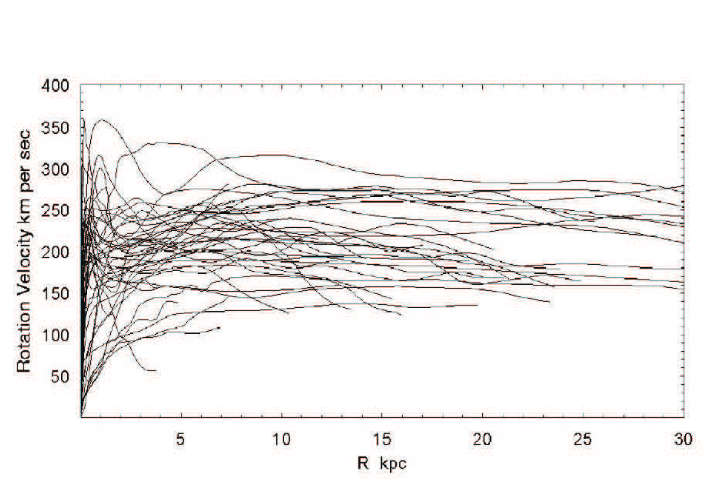
\includegraphics[scale=0.5]{rcurve.png}


\textbf{Figure:} \textit{ Rotation curves of spiral galaxies obtained by combining CO data for
the central regions, optical for disks, and HI for the outer disk and halo (Sofue et
al. 1999).} \cite{rcurve}
\end{center}

This suggests that ``$M$" should depend on ``$r$" when ``$r$" is sufficiently large\cite{rcurve}. Again we write $$\frac{v^2}{r}=\frac{GM(r)}{r^2}$$. $$\Rightarrow M(r)\propto r$$ as ``$v$" is constant. Now let density be ``$\rho(r)$".So $\int\rho(r)d^3r=M(r)$. Now we can see that if $\rho(r)\propto \frac{1}{r^2}$ then the condition $M(r)\propto r$ is fulfilled. From this, it is deduced that most of the mass lies outside the visible disk. An extended dark halo can not be seen as it does not interact with electromagnetic waves. It has different physical behavior from luminous matter which collapsed into the disk. Simulations of cold, collisionless DM predict that visible galaxies are embedded in extended dark matter halos, with densities approximately described by NFW or Einasto profiles.\\



\subsection{Acoustic oscillation}
 
  
  
 
Before the universe was about 300,000 years old, the universe was hot and dense. The universe was opaque. Radiation and matter were tightly glued together.  Photon had enough energy to excite an electron so that it could not form an atom. Thus frequent Compton scattering resulted in a shorter mean free path of the photon. Electrons and protons had electromagnetic interaction.  This state is called a photon-baryon fluid. Now during this epoch, gravity was compressing the fluid but the pressure of radiation was resisting it. It resulted in acoustic oscillations. So these oscillations existed because of the gravitational potential well. Now it is believed that the potential wells were not isolated. It is believed that structures in the universe were seeded by random quantum fluctuation. A period of rapid expansion, called ``inflation", is thought which caused these quantum fluctuations to be stretched into cosmic scales. These fluctuations in the energy density imply fluctuations in the local gravitational potential.  Regions of high density generate potential wells. Regions of low density generate potential hills. This modifies the picture of acoustic oscillations. The inflationary epoch lasted from $10^{-36}$ seconds after the Big Bang singularity to some time between $10^{-33}$ to $10^{-32}$ seconds after the singularity. \cite{whu} \\

When the universe was about 300,000 years old and the temperature was around 3000K, atoms started to form. Then the universe became transparent. This is called recombination. The radiation was decoupled from the fluid and was getting cooler as the universe was expanding. Ten to twenty billion years later, the background radiation we see is the same radiation that was decoupled from the photon-baryon fluid. This is called Cosmic Microwave Background(CMB). So from CMB, we get information about that epoch. The information on quantum fluctuation at that time is imprinted on CMB. The CMB is anisotropic of 1 part in 100,000. \cite{whu} \\

The Cosmic Microwave Background told us what the large-scale fluctuations in the background look like. But the small-scale fluctuations are also very interesting.COBE( Cosmic Microwave Background Explorer) measured temperature ripples from the $10\; degree$ to $90\; degree$ scale. This scale is so large that there has not been enough time for structures to evolve.  Hence COBE sees the so-called initial conditions of the universe. At the degree scale, on the other hand, the process of structure formation imprints information in the ripples about conditions in the early universe. The angular wavenumber, called a multipole l, of the power spectrum is related to the inverse of the angular scale (l=100 is approximately 1 degree).\\
 %Recent experiments, notably the Boomerang and Maxima experiments, have shown that the power spectrum exhibits a sharp peak of exactly the right form to be the ringing or acoustic phenomena.\\

\begin{center}
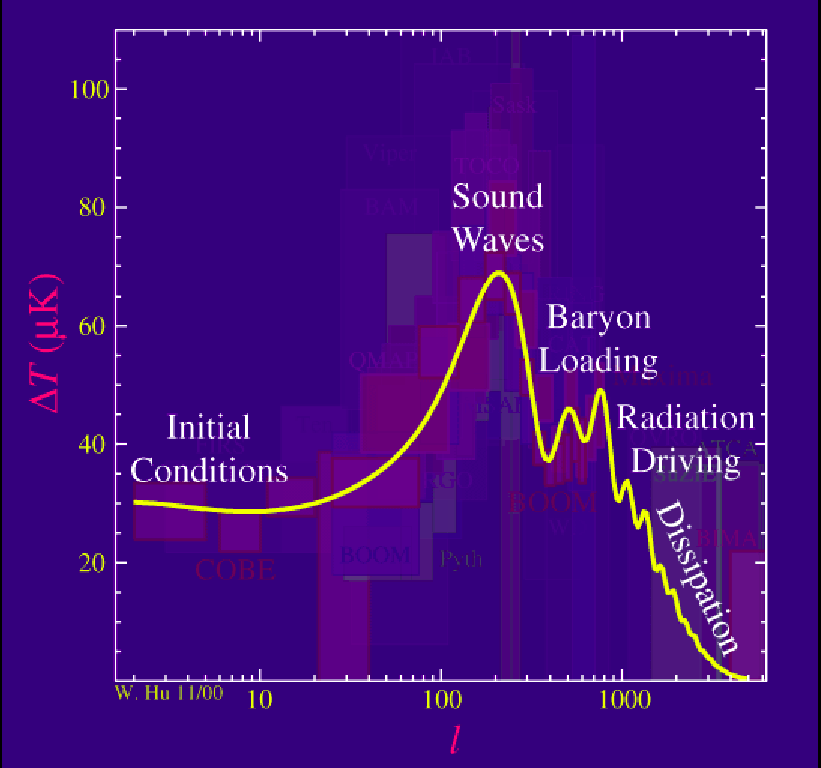
\includegraphics[scale=0.35]{deltvsl.png}\\
\textbf{Figure:} Temperature fluctuations of CMB vs multipole $l$ which is roughly 100/angles, observed by COBE.\cite{whu}
\end{center}


 The series of third and higher acoustic peaks is sensitive to the energy density ratio of dark matter to radiation in the universe.  Because the amount of radiation is known from the measured temperature of the CMB and the thermal history, under normal assumptions the third and higher acoustic peaks are sensitive to the dark matter density in the universe.%What happens is that if the radiation dominates the density, it is also what is making the gravitational potential in the first place.  Mathematically, the Poisson equation relates the overdensity of photons to the gravitational potential.  As pressure stops the radiation from further compression, the density fluctuation stabilizes leaving the gravitational potential to decay with the expansion of the universe. The decay happens when the fluid is in its most compressed state.  The fluid now sees no gravitational potential to fight against as it bounces back and the amplitude of the oscillations goes way up.\\
  
  %Because, this driving effect does not come into play once the density of the universe is dominated by the dark matter, we expect there to be a distinction between modes that started oscillating when the universe was radiation dominated and those that started oscillating when the universe was already matter dominated.  Because the density in radiation redshifts faster than matter due to the stretching of the photon wavelengths, the universe was radiation dominated only at its earliest epochs.  Finally, because modes of smaller wavelengths start oscillating first, it is the small-scale modes, or higher acoustic peaks, that feel this driving effect.  The upshot is that we expect a ramp-up of the amplitude of the peaks as we cross from low multipoles to high multipoles. Where this transition occurs tells us the energy density ratio of matter to radiation in the universe.\\
  \begin{center}
  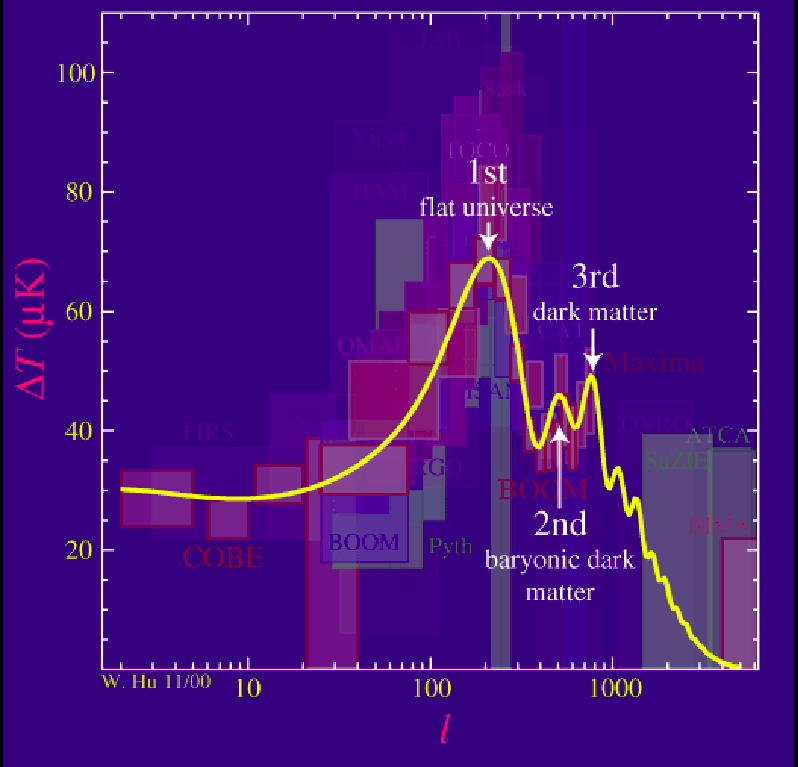
\includegraphics[scale=0.3]{PEAKS.png}\\
  \textbf{Figure:} Measure of abundances of elements in the universe from temperature fluctuations and its peaks.   \cite{whu}
  \end{center}
  
 % As we raise the physical density of the dark matter, $\Omega_mh^2$, the driving effect goes away at a given peak such that its amplitude decreases.  Although this effect changes the heights of all the peaks, it is only separable from the baryonic effects with at least three peaks.  Decreasing the matter density also affects the baryon loading since the dark matter potential wells go away leaving nothing for the baryons to fall into. Having a third peak that is boosted to a height comparable to or exceeding the second peak is an indication that dark matter dominated the matter density in the plasma before recombination.
 From this, we get an estimation of DM relic abundance. Recently Planck collaboration has given DM abundance $\Omega_{DM}h^2 \sim 0.120 \pm 0.001 $ \cite{pcolab}.\\

%Reproduced from \cite{whu}

\subsection{Gravitational Lensing}
Depending on matter concentration, the space-time metric gets changed. So when a photon passes by this area and follows the geodesic, it gets deflected. In many cases, this can be described in analogy to the deflection of light by lenses in optics. Now, observing this gravitationally lensed image, cosmologists can probe dark matter directly. This method is used to know more about its candidates, its properties, etc. There are some successful examples. \cite{glensing}

Now it is very clear that depending on the mass concentration of DM in a region, it will distort an image of a distant luminous object. Let the gravitational potential of this matter content be weak. For many of the cases of interest, one does not need to fully solve the general relativistic equation of motion for the coupled space-time and matter, because the bending of space-time by matter is small. So we can write a locally perturbed Minkowski metric in the following way: $$ds^2=\left(1+2\frac{\phi}{c^2}\right)c^2dt^2-\left(1-2\frac{\phi}{c^2}\right)dl^2$$ \cite{dmtheory1} \cite{dmtheory2}
There are different regimes: strong lensing, weak lensing, and microlensing. The distinction between these regimes depends on the positions of the source, lens, and observer and the mass and shape of the lens. 
\begin{itemize}
\item \textbf{Strong lensing:} The most extreme bending of light occurs when the lens is very massive and the source is close enough to it. In this case, light can travel in a different path to the observer and can create multiple images of the source. The first example of a double image was found in 1979, of the quasar. Given a set of images, one can try to reconstruct the lens mass distribution.


\item \textbf{Weak lensing:} In many cases the lens is not strong enough to form multiple images or arcs. However, the source can still be distorted: both stretched and magnified. If all sources are well-known, then one can deduce the properties of the lens.

\item \textbf{Microlensing:} In some cases the lensing is so small or faint that one does not see an image. The additional light bent towards the observer just means that the source appears brighter.
\end{itemize}

The lensing effect by DM is well known as they are the perfect matter to form a gravitational lens.\\

The most prolific evidence of DM was discovered using weak and strong gravitational lensing phenomena in the "Bullet cluster" or more formally in cluster 1E0657-56 \cite{dmtheory1}. Two galaxy clusters collided with each other about 4 billion light years away from Earth at the constellation Carina and created the Bullet cluster. It was the most energetic event after Big Bang. What happened is that the smaller cluster passed through the bigger one. From X-ray analyses, baryonic mass distribution was deduced, and weak and strong lensing phenomena gave the DM distribution. While passing through, the smaller cluster was colliding with the bigger one, and the shape of the smaller cluster became bullet-like due to the enormity of the collision. Evidence suggests that the collision was so enormous that the baryonic matter was distorted and displaced from its dark matter halo. But the dark matter halo just passed through each other. These phenomena not only give strong evidence of DM but also tells that DM is almost collisionless. \cite{dmtheory1}

\begin{center}
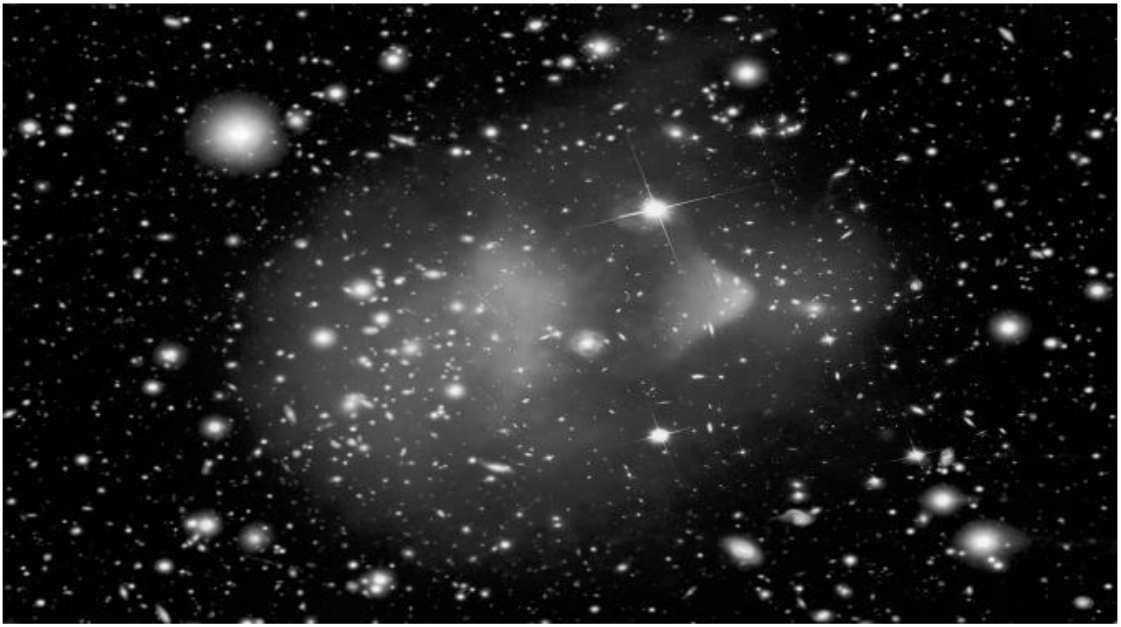
\includegraphics[scale=0.3]{bclstr.png}\\
\textbf{Figure:}The bullet cluster. Photo credit: NASA/CXC/CfA/ M.Markevitch et
al.; NASA/STScI; ESO WFI; Magellan/U.Arizona/ D.Clowe et al.;
NASA/STScI; Magellan/U.Arizona/D.Clowe et al.
\cite{dmtheory1}
\end{center}

 


\section{Types of Dark Matter}
The dark matter candidates are the relic particles whose comoving density becomes constant i.e. $n(t) a^3(t)= constant$ when the interaction rate $\Gamma$ of the dark matter particles falls below $H= \dot{a}/a$ of the Universe. The mass of the dark matter particle and the temperature of the Universe at the time of their decoupling determine whether the motion of the dark matter was relativistic or non-relativistic when they decoupled.\\

\textbf{Hot Dark Matter:} When the dark matter moves at relativistic speeds, it is termed hot dark matter. It has a mass less than the temperature of the Universe at a relevant time of the Universe. The hot dark matter candidates are generally of lighter mass.\\

\textbf{Cold Dark Matter:}If on the other hand the dark matter mass $m_\chi > T$, the temperature of the Universe at freeze-out, then these types of dark matter are known as cold dark matter (CDM). At the freeze-out, this type of dark matter particles were non-relativistic.


\section{Properties of Dark Matter}
All the probing mechanisms described in the previous section give us ideas about the characteristics of DM. This series of important results help us to invoke EFT. These results set some constraints to the DM degrees of freedom in our EFT. These results are:

\begin{itemize}
\item DM does not have electromagnetic interaction. But they have gravitational interaction. So they are electrically neutral.

\item The (dark+baryon) mass profiles of galaxies are very well modeled by
an isothermal profile $(\rho(r)\propto \frac{1}{r^2} )$. For clusters of galaxies, conclusions
are harder to draw without using weak gravitational lensing. However,
the discovery of radial arcs in the innermost regions of several clusters
of galaxies is difficult to reconcile with an internal shallow mass density
profile.

\item Most of the DM content is cold and collisionless.
\item The results of Planck collaborations suggest that DM in the universe is overwhelmingly non-baryonic. \cite{plcol}
\end{itemize}

\newpage

\chapter{ Matter relic density in the universe}

% \subsection{WIMP miracle}
% Let us assume that some kind of interaction keeps the DM particle in thermal equilibrium with the standard model particle. Let's also assume that DM can self-annihilate into SM particles. $$\chi\chi \rightarrow f\bar{f}$$ 
% the interaction rate $\Gamma$ corresponding to this scattering process just compensates the increasing scale factor at the point of decoupling $$\Gamma(T_{dec})=H(T_{dec})$$
% Let's assume that this interaction is set by the electroweak scale and for massive cold dark matter. To allow for an
% s-channel process in this scattering process, we use the Z-mass and Z-coupling in the corresponding annihilation cross section $$\sigma_{\chi\chi}(T<<m_\chi)\approx \frac{\pi\alpha^2m_\chi^2}{c_w^4m_Z^4}$$

%  Given the limited number of energy scales in our description we instead estimate very roughly $$\frac{1}{2}m_xv^2=T$$
%  $$\Rightarrow v=\sqrt{\frac{2T}{m_\chi}}$$
%  Now, if phase space distribution is $f(p)$ and $g$ is its internal degrees of freedom of a gas of particles, then $$n_{eq}(T)=\frac{g}{(2 \pi)^3} \int f(p)d^3p $$

%  We know phase space distribution: $$f(E)=\frac{1}{e^{\frac{E}{T}}\pm1}$$
%  We considered $k_B=1$ and $\mu=0$ i.e. zero chemical potential \footnote{ Basically, these particles will have other interactions which are stronger, that's why assuming their chemical potential to be zero is almost always a good one.}. Here "$+$" for Fermions and "$-$"for Bosons.
%  When $T<<m$, we can write,

%  $$n_{eq}(T) \cong g\sqrt[3]{\frac{mT}{2 \pi}}e^{-\frac{m}{T}}$$

%  In that case the condition of dark matter freeze-out is 

%  $$\Gamma=\sigma_{\chi \chi}v n_\chi$$

%  $$\Rightarrow H= \sigma_{\chi \chi}\sqrt{\frac{2T_{dec}}{m_\chi}} g \left(\frac{mT}{2 \pi}\right)^{\frac{3}{2}} e^{-\frac{m_\chi}{T}} $$
%  To go further we need the expression for $H$. Our universe is described by the FRW model. Now, in this framework, it is easy to show from the scale factor, that 

%  $$H=\frac{\pi\sqrt{g_{eff}}}{\sqrt{90}}\frac{T^2}{M_{PI}}$$ 

% Therefore, we can write,

%  $$\sigma_{\chi \chi}\frac{m_\chi T_{dec}^2}{\pi^{\frac{3}{2}}} e^{-x_{dec}} =  \frac{\pi}{3 \sqrt{10} M_{PI}} \sqrt{g_{eff} T_{dec}^2}$$

%  Here, we set the number of relevant degrees of freedom of the dark matter agent to $g = 2$, corresponding for example to a complex scalar or a Majorana fermion and $x_{dec}=\frac{m_{\chi}}{T}$.
%  Now, from this we get $e^{-x_{dec}}$. It is used to compute $n_{eq}$. This information is used to compute $\rho_{\chi \chi}$ from following relation: 


%  $$\rho_\chi(T_0)=m_\chi n_\chi(T_{dec})\left(\frac{a(T_{dec})}{a(T_0)}\right)$$

%  Then, all we have to do is use the following relation to compute the abundance of the matter:

%  $$\Omega_\chi h^2= \frac{\rho_\chi(T_0) h^2}{3 M_{PI}^2 H_0^2}$$

%  Now computation from this method gives the same abundance as the DM abundance. The result it gives is

%  $$\Omega_\chi h^2 \approx 0.12 \left(\frac{13 GeV}{m_\chi}\right)^2$$ 

%  This outcome is usually referred to as the WIMP miracle\cite{dmtheory1} \cite{dmtheory2}:  if we assume a dark matter agent with an electroweak-scale mass and an annihilation process mediated by the weak interaction, the predicted relic density comes out exactly as measured. Here, we need to recapitulate where this DM mass dependence comes from. This mass dependence comes from the general cross-section we considered. Our original assumption is $m_\chi < m_z$, which is not perfectly fulfilled, but also not completely wrong. It makes the point. Some of the assumptions we made in this non-relativistic and hence multi-scale calculation are not that convincing. So we should check this result from another perspective i.e. from thermal freeze out.\\


\section{Boltzmann Equation}
	From much of the early history of the universe, most of the constituents were in thermal equilibrium. But there are many examples where some constituents decoupled from others and departed from thermal equilibrium. It is easy to study matter evolution before decoupling and after decoupling. But around the epoch of decoupling, the study of evolution is challenging. We are interested in the decoupling of the relic WIMP. Now we have already mentioned that roughly the criterion for a particle species to be either coupled or decoupled involves the comparison of the interaction rate of the particle, $\Gamma$, with the expansion rate of the Universe, $H$ \cite{kolbbook}: 
	
$$\Gamma \gtrsim H \;\;\; \;(Coupled) \label{coupled} $$ 
$$\Gamma \lesssim H \;\;\;\; (Decoupled)  \label{decoupled}$$	
	
	
	
	Let us assume that some kind of interaction keeps the DM particle in thermal equilibrium with the standard model particle. Let's also assume that DM can self-annihilate into SM particles. $$\chi\chi \rightarrow f\bar{f}$$ 

Now, if phase space distribution is $f(p)$ and $g$ is its internal degrees of freedom of a gas of particles, then $$n_{eq}(T)=\frac{g}{(2 \pi)^3} \int f(p)d^3p $$
	
	
	
We know phase space distribution: $$f(E)=\frac{1}{e^{\frac{E}{T}}\pm1}$$
  We considered $k_B=1$ and $\mu=0$ i.e. zero chemical potential \footnote{ Basically, these particles will have other interactions which are stronger, that's why assuming their chemical potential to be zero is almost always a good one.}. Here "$+$" for Fermions and "$-$"for Bosons.
  When $T<<m$, we can write,

  $$n_{eq}(T) \cong g\sqrt[3]{\frac{mT}{2 \pi}}e^{-\frac{m}{T}}$$

  In that case, the condition of dark matter freeze-out is 

  $$\Gamma=\sigma_{\chi \chi}v n_\chi$$

 
  To go further we need the expression for $H$. Our universe is described by the FRW model. Now, in this framework, it is easy to show from the scale factor, that 

  $$H=\frac{\pi\sqrt{g_{eff}}}{\sqrt{90}}\frac{T^2}{M_{PI}}$$ 

 
	
	
	
	
	
	
	
	

Here, $\Gamma < H$, this condition is also known as freeze out. To study decoupling, one needs to study the evolution of the phase space distribution function $f(p^\mu, x^\mu)$. This is governed by the Boltzmann equation, which can be written as 

$$\hat{L}[f]=\hat{C}[f]$$

where $\hat{C}$ is the collision operator and $\hat{L}$ is the Liouville operator. The covariant, relativistic generalization of the Liouville operator is:

\begin{equation}
\hat{L} \equiv p^\alpha \frac{\partial}{\partial x^\alpha}-\Gamma^\alpha_{\; \beta \gamma} p^\alpha p^\gamma \frac{\partial}{\partial p^\alpha}
\end{equation}

For the FRW model of the Universe, the phase space density is spatially homogeneous and isotropic. So, it is only a function of energy and time i.e. $p^0$ and   $x^0$. The FRW metric is 

$$ds^2=dt^2-a^2(t)(dx^2+dy^2+dz^2) $$ \cite{gwald}

Here, $x^0=t$, $x^1=x$, $x^2=y$ and $x^3=z$. From this metric computing the connection coefficients, we get \cite{gwald}

$$\Gamma^0_{\;\;11}=\Gamma^0_{\;\;22}=\Gamma^0_{\;\;33}=a
\dot{a}$$

$$\Gamma^1_{\;\;10}=\Gamma^1_{\;\;01}=\Gamma^2_{\;\;20}=\Gamma^2_{\;\;02}=\Gamma^3_{\;\;30}=\Gamma^3_{\;\;03}=\frac{\dot{a}}{a}$$

Now consider this with the fact that the phase space distribution is only a function of energy and time, we get,


$$\hat{H}[f]=p^0 \frac{\partial f(E,t)}{\partial x^0}-\Gamma^0_{\;11} \;p^1 p^1 \frac{\partial f(E,t)}{\partial p^0}-\Gamma^0_{\;22} \;p^2 p^2 \frac{\partial f(E,t)}{\partial p^0}-\Gamma^0_{\;33} \;p^3 p^3 \frac{\partial f(E,t)}{\partial p^0}$$

$$=E \frac{\partial f(E,t)}{\partial t}- a\dot{a}\left((p^1)^2+(p^2)^2+(p^3)^2\right) \frac{\partial f(E,t)}{\partial E} $$

Now, at this point, we need to use $$g_{\mu \nu}p^\mu p^\nu= m^2$$.
From this relation, it can be shown that,
$$(p^1)^2+(p^2)^2+(p^3)^2= \frac{(\mid\vec{p}\mid)^2}{a^2(t)}$$ 
Now the Liouville operator becomes:


$$\hat{L}[f]=E\frac{\partial f(E,t)}{\partial t}- \frac{\dot{a}}{a} \left(\mid \vec{p}\mid \right)^2 \frac{\partial f(E,t)}{\partial E}$$

Therefore,



\begin{align*}
& E\frac{\partial f(E,t)}{\partial t}- \frac{\dot{a}}{a} \left(\mid \vec{p}\mid\right)^2 \frac{\partial f(E,t)}{\partial E} =\hat{C}[f]\\
& \Rightarrow \frac{\partial f(E,t)}{\partial t}- \frac{\dot{a}}{a} p \frac{\partial f(E,t)}{\partial p} = \frac{1}{E} \hat{C}[f]\\
& \Rightarrow \frac{\partial}{\partial t} \left( \frac{g}{(2 \pi)^3} \int d^3p f(E,t) \right)- \frac{\dot{a}}{a} \frac{g}{(2 \pi)^3} \int d^3p \frac{\partial f(E,t)}{\partial p} p = \frac{g}{(2 \pi)^3} \int \frac{1}{E} \hat{C}[f] d^3p \\
& \Rightarrow \frac{\partial}{\partial t} \left( \frac{g}{(2 \pi)^3} \int d^3p f(E,t) \right)- \frac{\dot{a}}{a} \frac{g}{(2 \pi)^3} \left[\int \int \frac{\partial f(E,t)}{\partial p} p\; \; p^2dp\;d\Omega \right] \\
&\;\;\;\;\;\;\;\;\;\;\;\;\;\;\;\;\;\;\;\;\;\;\;\;\;\;\;\;\;\;\;\;\;\;\;\;\;\;\;\;\;\;\;\;\;\;\;\;\;\;\;\;\;\;\;\;\;\;\;\;\;\;\;\;\;\;\;\;\;\;\;\;\;\;\;\;\;\; = \frac{g}{(2 \pi)^3} \int \frac{1}{E} \hat{C}[f] d^3p\\
& \Rightarrow \frac{\partial}{\partial t} \left( \frac{g}{(2 \pi)^3} \int d^3p f(E,t) \right)- \frac{\dot{a}}{a} \frac{g}{(2 \pi)^3} \left[4 \pi \int \frac{\partial f(E,t)}{\partial p} p^3dp \right] \\
&\;\;\;\;\;\;\;\;\;\;\;\;\;\;\;\;\;\;\;\;\;\;\;\;\;\;\;\;\;\;\;\;\;\;\;\;\;\;\;\;\;\;\;\;\;\;\;\;\;\;\;\;\;\;\;\;\;\;\;\;\;\;\;\;\;\;\;\;\;\;\;\;\;\;\;\;\;\;\;\;\;\;\;\;\;= \frac{g}{(2 \pi)^3} \int \frac{1}{E} \hat{C}[f] d^3p\\
& \Rightarrow \frac{\partial}{\partial t} \left( \frac{g}{(2 \pi)^3} \int d^3p f(E,t) \right)- \frac{\dot{a}}{a} \frac{g}{(2 \pi)^3} \; 4 \pi  \left[p ^3 \int \frac{\partial f(E,t)}{\partial p}dp- \int(3p^2f)dp \right]\\
&\;\;\;\;\;\;\;\;\;\;\;\;\;\;\;\;\;\;\;\;\;\;\;\;\;\;\;\;\;\;\;\;\;\;\;\;\;\;\;\;\;\;\;\;\;\;\;\;\;\;\;\;\;\;\;\;\;\;\;\;\;\;\;\;\;\;\;\;\;\;\;\;\;\;\;\;\;\;\;\;\;\;\;\;\;\; = \frac{g}{(2 \pi)^3} \int \frac{1}{E} \hat{C}[f] d^3p \\
& \Rightarrow \frac{\partial}{\partial t} \left( \frac{g}{(2 \pi)^3} \int d^3p f(E,t) \right)-3 \frac{\dot{a}}{a} \frac{g}{(2 \pi)^3} \left[\int \int f(E,t) p^2dpd\Omega \right] \\
&\;\;\;\;\;\;\;\;\;\;\;\;\;\;\;\;\;\;\;\;\;\;\;\;\;\;\;\;\;\;\;\;\;\;\;\;\;\;\;\;\;\;\;\;\;\;\;\;\;\;\;\;\;\;\;\;\;\;\;\;\;\;\;\;\;\;\;\;\;\;\;\;\;\;\;\;\;\;\;\;\;\;\;\;\;= \frac{g}{(2 \pi)^3} \int \frac{1}{E} \hat{C}[f] d^3p\\
& \Rightarrow \frac{\partial}{\partial t} \left( \frac{g}{(2 \pi)^3} \int d^3p f(E,t) \right)-3 \frac{\dot{a}}{a} \frac{g}{(2 \pi)^3} \left(\int f(E,t) d^3p \right) = \frac{g}{(2 \pi)^3} \int \frac{1}{E} \hat{C}[f] d^3p\\
&\Rightarrow \frac{\partial n}{\partial t} + 3 \frac{\dot{a}}{a}n=\frac{g}{(2 \pi)^3} \int \frac{1}{E} \hat{C}[f] d^3p \label{b1}
\end{align*}


We have already simplified the Boltzmann transport equation. The only thing remaining here is to simplify the collision term of the equation for the $2 \rightarrow 2$ process. The collision term for the process $\psi+a \longleftrightarrow i + j$ is given by \cite{kolbbook}
\begin{multline*}
 \frac{g}{(2 \pi)^3} \int \hat{C}[f] \frac{d^3 p_\psi}{E_\psi} = \int d \Pi_\psi d \Pi_a d \Pi_i d \Pi_j (2 \pi)^4 \delta^4(p_\psi + p_a - p_i - p_j)\\
 \left[\mid \mathcal{M}\mid ^2_{i+j \rightarrow \psi+a} f_i f_j (1 \pm f_\psi)(1 \pm f_a)-[\mid \mathcal{M}\mid ^2_{\psi+a \rightarrow i+j} f_a f_\psi (1 \pm f_i)(1 \pm f_j) \right]
\end{multline*} \label{b2}

(+) sign applies to bosons and (-) sign applies to fermions; and 

$$d \Pi \equiv \frac{g}{(2 \pi)^3} \frac{d^3p}{2E}$$.
In this case, we can simplify this demanding CP invariance, which implies 
$$\mid \mathcal{M}\mid ^2_{i+j \rightarrow \psi+a}= \mid \mathcal{M}\mid ^2_{\psi+a \rightarrow i+j}=\mid \mathcal{M} \mid^2 $$

In the absence of Bose condensation or Fermi degeneracy, the blocking and stimulated emission factors can be ignored, $1+f \simeq 1$, and $f_i (E_i) = e^{-E_i/T}$ for all species in kinetic equilibrium. Now, with these assumptions, the Boltzmann equation may be cast in the familiar form

$$\dot{n_\psi}+3 H n_\psi=-\int d \Pi_\psi d \Pi_a d \Pi_i d \Pi_j (2 \pi)^4 \mid \mathcal{M} \mid^2 \delta^4(p_\psi + p_a - p_i - p_j) [f_a f_\psi- f_i f_j]$$
Now let us study the following annihilation process

$$\chi \chi \longleftrightarrow \psi \bar{\psi} $$
We need to note here that we considered the chemical potential of the product zero. In this case, we can write


\begin{multline*}
\dot{n_\chi}+3Hn_\chi = -\int \int \int \int \frac{g_\chi}{(2 \pi)^3} \frac{d^3p^\prime_\chi}{2E^\prime_\psi} \frac{g_\chi}{(2 \pi)^3} \frac{d^3p_\chi}{2E_\chi} \frac{g_\psi}{(2 \pi)^3} \frac{d^3p_\psi}{2E\psi} \frac{g_{\bar{\psi}}}{(2 \pi)^3} \frac{d^3p_{\bar{\psi}}}{2E_{\bar{\psi}}} (2 \pi)^4 \mid \mathcal{M} \mid^2 \\
\delta^4(p_\chi + p^\prime_\chi - p_\psi - p_{\bar{\psi}})\left[f_\chi f_\chi- f_\psi f_{\bar{\psi}} \right] \\
= -\int \int \int \int \frac{g_\chi}{(2 \pi)^3} \frac{d^3p ^\prime_\chi}{2E^\prime_\psi} \frac{g_\chi}{(2 \pi)^3} \frac{d^3p_\chi}{2E_\chi} \frac{g_\psi}{(2 \pi)^3} \frac{d^3p_\psi}{2E\psi} \frac{g_{\bar{\psi}}}{(2 \pi)^3} \frac{d^3p_{\bar{\psi}}}{2E_{\bar{\psi}}} (2 \pi)^4 \mid \mathcal{M} \mid^2 \\
\delta^4(p_\chi + p^\prime_\chi - p_\psi - p_{\bar{\psi}})\left[f_\chi f_\chi-e^{-(E_\psi+E_{\bar{\psi}})/T} \right]\\
= -\int \int \int \int \frac{g_\chi}{(2 \pi)^3} \frac{d^3p ^\prime_\chi}{2E^\prime_\psi} \frac{g_\chi}{(2 \pi)^3} \frac{d^3p_\chi}{2E_\chi} \frac{g_\psi}{(2 \pi)^3} \frac{d^3p_\psi}{2E\psi} \frac{g_{\bar{\psi}}}{(2 \pi)^3} \frac{d^3p_{\bar{\psi}}}{2E_{\bar{\psi}}} (2 \pi)^4 \mid \mathcal{M} \mid^2 \\
\delta^4(p_\chi + p^\prime_\chi - p_\psi - p_{\bar{\psi}})\left[f_\chi f_\chi-e^{-(E_\chi+ E^\prime _\chi)/T} \right]\\
=-\int \int \int \int \frac{g_\chi}{(2 \pi)^3} \frac{d^3p ^\prime_\chi}{2E^\prime_\psi} \frac{g_\chi}{(2 \pi)^3} \frac{d^3p_\chi}{2E_\chi} \frac{g_\psi}{(2 \pi)^3} \frac{d^3p_\psi}{2E\psi} \frac{g_{\bar{\psi}}}{(2 \pi)^3} \frac{d^3p_{\bar{\psi}}}{2E_{\bar{\psi}}} (2 \pi)^4 \mid \mathcal{M} \mid^2 \\
\delta^4(p_\chi + p^\prime_\chi - p_\psi - p_{\bar{\psi}})\left[f_\chi f_\chi- f^{EQ}_\chi f^{EQ}_\chi \right]\\
=-<\sigma  v > \left[ n^2_\chi -(n^{EQ}_\chi)^2 \right]
\end{multline*}
Now the final equation we get is,

\begin{equation}
\frac{dn_\chi}{dt}+3Hn_\chi = -<\sigma  v> [ n^2_\chi -(n^{EQ}_\chi)^2]
\end{equation}

After decoupling we know that the number density of a species of particles which are not being created or destroyed is $n(t) \propto 1/ a^3(t)$. This motivates us to study the evolution of the number density of particles per comoving volume. We can assign another variable $Y(t)$. Then the equation can be re-written as,


\begin{align}
&\frac{1}{a^3(t)} \frac{d}{dt} (n_\chi a^3(t))= -<\sigma v> [n^2_\chi-(n^{EQ}_\chi)^2] \\
&\Rightarrow \frac{dY}{dt} = -<\sigma v> T^3(t) [Y^2- (Y_{EQ})^2] \label{yeqn}
\end{align}

Now to solve this we replace the time with some other variable describing the history of
the Universe. We switch variables to $x = m\chi /T$. For the Jacobian we assume that most of the dark matter
decoupling happens with $\rho_r >> \rho_m $; in the early, radiation-dominated Universe we can link the time and $x$ through,  \cite{dmtheory4}

$$\frac{1}{2t} = \frac{H(x=1)}{x^2}$$

$$\Rightarrow \frac{dx}{dt}= \frac{H(x=1)}{x}$$

Therefore, we can write,
 $$\frac{dY}{dx} =\frac{ \frac{dY}{dt}}{\frac{dx}{dt}} $$
 $$=- \frac{x}{H(x=1)} <\sigma v> T^3(t) [Y^2- (Y_{EQ})^2]$$

$$=-\frac{x}{H(x=1)} <\sigma v> \frac{m^3_\chi}{x^3} [Y^2- (Y_{EQ})^2]$$
$$= - \frac{<\sigma v> m^3_\chi}{H(x=1) x^2}\;\; [Y^2(x)- (Y_{EQ}(x))^2] $$
$$=- \frac{\lambda(x)}{x^2}\; \; [Y^2(x)- (Y_{EQ}(x))^2] $$
To analytically solve this Boltzmann equation we make two approximations \cite{dmtheory4}: first, the equilibrium density drops like $e^{−x}$ towards later times or increasing $x$. Assuming that the actual number density $n_{\chi}(x)$ drops more slowly, we can safely approximate the Boltzmann equation \ref{yeqn} by
\begin{equation}
\frac{dY}{dx}=-\frac{\lambda(x)}{x^2} \; Y^2(x)
\end{equation}

Second, we can estimate $\lambda(x)$ by expanding the thermally averaged annihilation WIMP cross-section for small velocities. So,
\begin{align*}
& \lambda(x) = \frac{m^3_\chi <\sigma v>}{H(x=1)}\\
& =\frac{\sqrt{90} M_{PI}\; m_x}{\pi \sqrt{g_{eff}}} <\sigma v> (x)\\
&= \frac{\sqrt{90} M_{PI}\; m_x}{\pi \sqrt{g_{eff}}} \; \sigma v + \mathcal{O}(v^2) \\
& \approx \frac{\sqrt{90} M_{PI}\; m_x}{\pi \sqrt{g_{eff}}} \sqrt{\frac{2}{x}} \frac{\pi \alpha^2 m^2_\chi}{c^4_w m^4_z} \equiv \frac{\bar{\lambda}}{\sqrt{x}}
\end{align*}

The value $\bar{\lambda}(x)$ depends on $x$ independently through $g_{eff}$, so we can assume it to be constant as long as $g_{eff}$ does not change much. Under this assumption, we can then solve the Boltzmann equation with the simple substitution
$\bar{Y} = 1/Y$. Therefore, 

$$\frac{d\bar {Y} }{dx}= \frac{\bar{\lambda}}{x^{5/2}}$$

we know that thermal WIMPs have masses well above $10 GeV$, which corresponds to $g_{eff} \approx 100$.
This value only changes once the temperature reaches the bottom mass and then drops to $g_{eff} \approx 3.6$ today. This allows us to separate the leading effects driving the dark matter density into the decoupling phase described by the Boltzmann equation and an expansion phase with its drop in $g_{eff}$. For the first phase, we can just integrate the Boltzmann equation for constant $g_{eff}$ starting just before decoupling $(x_{dec} )$ and to a point $x^\prime_{dec}>> x_dec$ after decoupling but above the bottom mass,

\begin{align*}
& \frac{1}{Y(x^\prime_{dec})}- \frac{1}{Y(x_{dec})}\\
& \bar{Y}(x_{dec})- \bar{Y}(x_{dec}) = -\frac{\lambda}{(x^\prime_{dec})^{3/2}} + \frac{\lambda}{(x_{dec})^{3/2}}
\end{align*}

From the form of the Boltzmann equation in Eq.$3$, we see that $Y (x)$ drops rapidly with increasing $x$. If we
choose $x^\prime_{dec} >> x_{dec}$ it follows that $Y(x\prime_{dec} ) << Y(x_dec )$ and hence
\begin{align*}
&\frac{1}{Y(x^\prime_{dec})} =\frac{\bar{\lambda}}{x^{3/2}}\\
&\Rightarrow Y(x^\prime_{dec}) =\frac{x_{dec}}{\lambda}\\
&\Rightarrow Y(x^\prime_{dec})= x_{dec} \; \; \frac{\pi \sqrt{g_{eff}}}{\sqrt{90} M_{PI} m_\chi} \frac{1}{<\sigma v>}
\end{align*}

In this expression, $g_{eff}$ is evaluated around the point of decoupling. For the second, expansion phase we can write
\begin{align*}
\rho_\chi(T_0)= m_\chi n_\chi(T_0)\\
& = m_\chi Y(x^\prime_{dec})\; \;\; (T^\prime_{dec})^3 \left( \frac{a(T^\prime_{dec})}{a(T_0)}\right)^3\\
&= m_\chi Y(x^\prime_dec) T^3_0 \frac{g_{eff}(T_0)}{g_{eff}(T^\prime_{dec})}
\end{align*}
For the properly normalized relic density, this means

\begin{align*}
& \Omega_\chi h^2 = m_\chi Y(x^\prime_dec) T^3_0 \frac{g_{eff}(T_0)}{g_{eff}(T^\prime_{dec})} \frac{h^2}{3 M^2_{PI} H^2_0}\\
& = m_\chi x_{dec} \; \; \frac{\pi \sqrt{g_{eff}}}{\sqrt{90} M_{PI} m_\chi} \frac{1}{<\sigma v>} T^3_0 \frac{g_{eff}(T_0)}{g_{eff}(T^\prime_{dec})} \frac{h^2}{3 M^2_{PI} H^2_0}
\end{align*}


Now this result illustrates an interesting feature of freeze-out. The relic density of $\chi$'s is inversely proportional to the cross-section and mass of the particle. The smaller the annihilation cross-section, the greater the relic abundance - the weak prevail.
 Now the result i.e. the relic abundance for weak scale interactions from this formula is the same as the abundance of the Dark Matter. This is called the WIMP miracle.
 
 Let us briefly recapitulate our argument which through the Boltzmann equation leads us to the WIMP miracle: we start with a $2 \longrightarrow 2$ scattering process linking dark matter to Standard Model particles through a so-called mediator, which can for example be a weak boson. This allows us to compute the dark matter relic density as a function of the mediating coupling and the dark matter mass, and it turns out that a weak coupling fits perfectly.

\newpage

\chapter{Strategy for Dark Matter searches/detection}
There are essentially three different experimental methods to detect Dark Matter.

\textbf{Collider searches:} Extensive unsuccessful searches for the particle involved in supersymmetric models have been performed at particle accelerators throughout the world. No supersymmetric particle was found in this energy range. But this does not yet mean low energy supersymmetry is unlikely to exist since only a small portion of the allowed mass range under $1\; TeV$ has been explored. The EFT approach in this case is challenging. Because the center of mass energy in this case is high.

The experimental method in this case is simple. Two SM particles will collide with each other and there is a probability that the product will be DM particles. We will see them as missing energy in our experiments.

\begin{center}
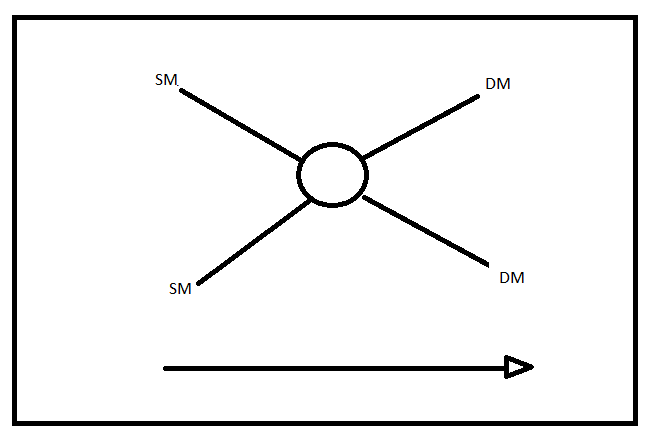
\includegraphics[scale=0.3]{collider_searches1.png}
\end{center}


\textbf{Direct Detection:} A satisfying solution to the Dark Matter problem would be the detection of WIMPs from our galactic halo as they move past and through Earth. This would also give us information about the local density of DM and establish that DM is non-baryonic cold dark matter. One of the two ways to probe this is direct detection.

A stream of DM particles passing through the earth would interact with nuclei weakly. As the particles are weakly interacting, most of them would pass right through the Earth unimpeded. In addition, if a WIMP does scatter off a nucleus, the deposited energy is in the $keV$ range. This is too small to notice except by very sensitive equipment. The interesting thing is the detection rates turn out to be within and just beyond the reach of current experimental efforts. 

Direct detection experiments aim to detect recoils of nuclei induced by interaction with DM particles. The main difficulties in these experiments come from the fact that the WIMP events are very rare and that there are similar backgrounds that deposit the same amount of energy more frequently. That is why the experiments operate deep underground where this background is screened off. The experiments operate their detectors at extremely low temperatures to keep thermal excitations low.

\begin{center}
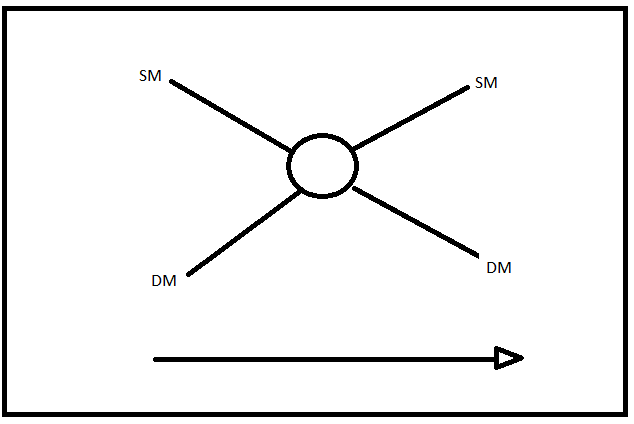
\includegraphics[scale=0.3]{Direct_detection1.png}
\end{center}

\textbf{Indirect detection:} A great deal of theoretical and experimental effort has gone into another potential way of detecting cold dark matter indirect detection. This detection method is theorized based on the fact that WIMPs will self-annihilate into SM particles. The product particles are less massive compared to the WIMPs. So, the energy spectrum of the SM particles is very high. That is why it is almost impossible to confuse them with other particles produced by other processes. Our potential theoretical framework for this method is EFT. 

\begin{center}
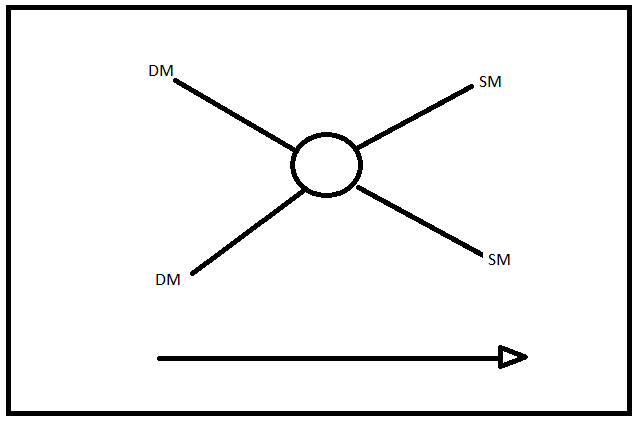
\includegraphics[scale=0.3]{indirect_detection1.png}
\end{center}

\newpage

\chapter{EFT of DM indirect detection}

\section{Effective Field Theory}

Effective field theory is a full-fledged quantum theory in a different scale of an underlying theory, sometimes called "full theory". To measure something quantitative from an experiment often we do not need to know the full underlying theory. It may happen that what we expect from the theory can be evaluated from an asymptotic limit of the full theory, so this result can be obtained from a different scale of parameters involved.
A layman's example is, an architect does not need to know how matter interacts with each other to build a bridge or buildings. All he/she needs to know is Newton's laws of motion and gravitation. Another example is QED is an effective field theory of the Standard Model.
An EFT is a quantum theory in its own right. We can compute S-matrix elements from its lagrangian. The final result which is experimentally measurable, we compute from this lagrangian has a finite error. Formally EFT results are an expansion of a parameter $\delta$. We terminate the expansion at $\delta^n$ and all the terms involving $n+1$ power and greater than that of delta go into the error part of that theory. This tells us that we can expand our interaction terms in terms of this parameter. Our theory gives us some constraints depending on the expansion coefficients and parameters. This tells us that to compare the results of our experiments we need to operate our experiments fulfilling all the conditions the theory demands.\\

In the framework of the EFT interaction terms in the lagrangian is written as an expansion of its degrees of freedom and some couplings and a term $\Lambda$. This $\Lambda$ is called the cut-off of our theory. The reason $\Lambda$ is called cut-off would be clear from power counting. Now effective field theories are the appropriate theoretical tool to describe low-energy physics, where low is defined concerning energy scale $\Lambda$. Now in this regime, we will be considering only relevant degrees of freedom. Although effective field theories contain an infinite
number of terms, renormalizability is not an issue since, at a given order in the energy expansion, the low-energy theory is specified by a finite number of couplings; this allows for an order-by-order renormalization \cite{eft1} \cite{eft2}. \\

The theoretical basis of effective field theory (EFT) can be formulated as a theorem \cite{eft2}:\\



For a given set of asymptotic states, perturbation theory with the most general Lagrangian containing all terms allowed by the assumed symmetries will yield the most general S-matrix elements consistent with analyticity, perturbative unitarity, cluster decomposition, and the assumed symmetries.

\textbf{Power counting:} Before we start describing the technical details of power counting and setting cut-off in our effective Lagrangian, we would specify the mass dimensions of some fields.
(Here $c=1$ and $\hbar = 1$, and spactime dimension $d=4$)
\begin{center}
Scalar fields$[\phi]= 1$\\
Fermionic fields $[\psi]= \frac{3}{2}$\\
Vector fields $[A_\mu]=1$\\
\end{center}

Now we write the EFT lagrangian as an expansion in powers of the operator dimension:


$$\mathscr{L}_{EFT}= \sum_{\mathscr{D}\geq 0} \frac{\mathscr{L}_\mathscr{D}}{\Lambda^{(\mathscr{D}-4)}}= \sum_{\mathscr{D}\geq 0 ,i} \frac{c_i^{(\mathscr{D})}\; \mathcal{O}_i^{(\mathscr{D})}}{\Lambda^{(\mathscr{D}-4)}}$$

where $\mathcal{O}_i^{(\mathscr{D})}$ are the allowed operators of dimension $\mathscr{D}$ . All operators of dimension $\mathscr{D}$
are combined into the dimension $\mathscr{D}$ Lagrangian $\mathscr{L}_\mathscr{D}$ . Here we take all the operators of arbitrarily high dimensions.
A scale $\Lambda$ has been introduced so that the coefficients $c_i$ are dimensionless. $\Lambda$ is the short-distance scale at which new physics occurs.
what is relevant for theoretical calculations and experimental measurements is the
product $c_\mathscr{D} \Lambda^{4-D}$, not $c_\mathscr{D}$ and $\Lambda^{4-D}$ separately. $\Lambda$ is a convenient device that makes it clear how to organize the EFT expansion.

We can write \cite{eft1} \cite{eft2}

$$\mathscr{L}_{EFT}=\mathscr{L}_{\mathscr{D}\leq 4}+\frac{\mathscr{L}_5}{\Lambda}+\frac{\mathscr{L}_6}{\Lambda^2}+\frac{\mathscr{L}_7}{\Lambda^3}+.....$$

$\mathscr{L}_{EFT}$ is given by an infinite series of terms of increasing operator dimension. An important point is that the $\mathscr{L}_{EFT}$ has to be treated as an expansion in powers of $1/\Lambda$.
If we try and sum terms to all orders, the EFT will break down.

 Let us consider a scattering amplitude $\mathcal{M}$
in space-time dimension $d=4$. If one works at some typical momentum scale $p$, then a single insertion of an operator of dimension $\mathscr{D}$ in the scattering graph gives a contribution to the amplitude of the order

$$\mathcal{M} \sim \left(\frac{p}{\Lambda} \right)^{\mathscr{D}-4}$$

by dimensional analysis. Insertion of a set
of higher dimension operators in a tree graph leads to an amplitude

$$\mathcal{M} \sim \left(\frac{p}{\Lambda} \right)^n$$
 with $n=\sum_i (\mathscr{D}_i - 4)$ . where the sum on $i$ is over all the inserted operators. This follows from dimensional analysis, as for a single insertion. This formula is known as the EFT power counting formula.
 To construct our operator we need the notion of power counting and setting cut-off.


\section{EFT operators}
In this thesis paper, we will be discussing the field theory part of DM detection. We will give a detailed discussion on computing cross-section. If that part is resolved then all we need is to put it in the equation we will later derive. We will compute it considering our DM candidate as a scalar field. Our target is to see whether our results depend on the velocity of the DM or not. Whether CTA can detect the signal or not will depend on the velocity suppression of the cross-section. If the non-relativistic cross-section depends on the velocity, then CTA can not detect it.\\

Now we need to construct the effective operators where DM will self-annihilate in SM particles, particularly in quarks, W-bosons, Z-boson, and photons. We need to also consider the operators to be SM invariant. We constructed the following operators which were also mentioned in  \cite{dmeft} :
\begin{center}
\begin{tabular}{|c|c|}
\hline
Label & Operators\\ \hline
$\mathcal{O}_1$ & $\frac{c}{\Lambda} \phi^2 \bar{q}q$\\ \hline
$\mathcal{O}_2$ & $\frac{c_1}{\Lambda^2} \phi^2 W_{\mu \nu a} W^{\mu \nu}_a$ \\ \hline

$\mathcal{O}_3$ & $\frac{c_2}{\Lambda^2} \phi^2 B_{\mu \nu} B^{\mu \nu}$\\ \hline
\end{tabular}
\end{center}
We will compute the cross section for the following annihilation processes from this operators: $ DM\; DM \longrightarrow q \bar{q}\; (from\; \mathcal{O}_1), \; \; DM\; DM \longrightarrow W^+W^-(From\; \mathcal{O}_2), \; \; \\
DM\; DM \longrightarrow ZZ (from\; \mathcal{O}_2 \; and\; \mathcal{O}_3 ), \; \; DM\; DM \longrightarrow \gamma Z (from\; \mathcal{O}_2 \; and\; \mathcal{O}_3 ) , \; \; \\ DM\; DM \longrightarrow \gamma  \gamma (from\; \mathcal{O}_2  \; and\; \mathcal{O}_3 )$.

All the combinatorial factors for $DM$ i.e. $\phi$ field were absorbed here in the dimensionless coupling constants.
Now before we start computing we need to reduce these effective operators for $2 \longrightarrow 2$ processes.\\

\textbf{$\mathcal{O}_2 $:} In case of this operator we need to reduce $W_{\mu \nu a} W^{\mu \nu}_a$.

We will write them in their component fields.

Therefore we get:

\begin{align*}
&W_{\mu \nu a} W^{\mu \nu}_a \\
& = (\partial_\mu W_{\nu a} - \partial_\nu W_{\mu a} + i \epsilon_{abc} W_{\mu b} W_{\nu c}) (\partial^\mu W^\nu_a- \partial^\nu W^\mu_a+ i \epsilon_{adl} W^\mu_d W^\nu_l)
\end{align*}

From $\mathcal{O}_2 $:

\begin{align*}
& \frac{c_1}{\Lambda^2} \phi^2 W_{\mu \nu a} W^{\mu \nu}_a \\
&=\frac{c_1}{\Lambda^2} \phi^2(\partial_\mu W_{\nu a} - \partial_\nu W_{\mu a} + i \epsilon_{abc} W_{\mu b} W_{\nu c}) (\partial^\mu W^\nu_a- \partial^\nu W^\mu_a+ i \epsilon_{adl} W^\mu_d W^\nu_l)\\
\end{align*}



For $2 \longrightarrow 2$ processes:



\begin{align*}
&\frac{c_1}{\Lambda^2} \phi^2 (\partial^\mu W^\nu_a\; \partial_\mu W_{\nu a} -\partial^\mu W^\nu_a\; \partial_\nu W_{\mu a}- \partial^\nu W^\mu_a\; \partial_\mu W_{\nu a} + \partial^\nu W^\mu_a\; \partial_\nu W_{\mu a})\\
&=\frac{c_1}{\Lambda^2} \phi^2 (2\; \partial^\mu W^\nu_a\; \partial_\mu W_{\nu a}-2\; \partial^\mu W^\nu_a\; \partial_\nu W_{\mu a})\\
&=\frac{2c_1}{\Lambda^2} \phi^2 (\partial^\mu W^\nu_a\; \partial_\mu W_{\nu a}- \partial^\mu W^\nu_a\; \partial_\nu W_{\mu a})
\end{align*}

From $\mathcal{O}_3 $:

\begin{align*}
&\frac{c_2}{\Lambda^2} \phi^2 B_{\mu \nu} B^{\mu \nu}\\
&=\frac{c_2}{\Lambda^2} \phi^2 (\partial_\mu B_\nu - \partial_\nu B_\mu) (\partial^\mu B^\nu - \partial^\nu B^\mu)\\
& =\frac{c_2}{\Lambda^2} \phi^2 (\partial_\mu B_\nu\; \partial^\mu B^\nu - \partial_\mu B_\nu\; \partial^\nu B^\mu - \partial_\nu B_\mu\; \partial^\mu B^\nu +\partial_\nu B_\mu\; \partial^\nu B^\mu)\\
& =\frac{2c_2}{\Lambda^2} \phi^2 (\partial_\mu B_\nu\; \partial^\mu B^\nu-\partial_\mu B_\nu\; \partial^\nu B^\mu)
\end{align*}

Now the operators have the following form:

\begin{equation}
\mathcal{O}_2 : \frac{2c_1}{\Lambda^2} \phi^2 (\partial^\mu W^\nu_a\; \partial_\mu W_{\nu a}- \partial^\mu W^\nu_a\; \partial_\nu W_{\mu a}) \label{wwop}
\end{equation}

\begin{equation}
\mathcal{O}_3 :\frac{2c_2}{\Lambda^2} \phi^2 (\partial_\mu B_\nu\; \partial^\mu B^\nu-\partial_\mu B_\nu\; \partial^\nu B^\mu) \label{zzop}
\end{equation}

If we put $a=1\; and\; 2$ in \ref{wwop} we will get $\phi\phi \longrightarrow W^+ W^-$.
 
 
\section{Dark Matter Indirect Detection}

In principle, DM can annihilate or decay into any SM particles. The final state of the annihilation process is stable particles which we can detect.

These produced SM particles from this annihilation process will produce secondary particles.

\begin{align*}
DM\;\; DM \longrightarrow& W^+ W^-, ZZ, \gamma\; \gamma, \gamma Z\\
&W^+ \longrightarrow l^+\; \nu,\; Z \longrightarrow l^+ \; l^-\\
&l^+ \longrightarrow l^+ \gamma...... (Secondary\;\; particles/ \;\; emission)
\end{align*}


We focus on primary $\gamma$'s coming from  $DM\; DM \longrightarrow \gamma Z , \; \; \\ DM\; DM \longrightarrow \gamma  \gamma $ cannels and secondary $\gamma$'s coming from $DM\;DM \longrightarrow q \bar{q}\; , \; \; \\ DM\; DM \longrightarrow W^+W^-, \; \;
DM\; DM \longrightarrow ZZ$ channels.

\textbf{Neutral particles :} Let us consider particles that travel to us in straight lines. In general, we have a two-dimensional view of the sky, although we may discern the distance at which a particle was produced as we have the notion of redshift.
What we observe is the number of particles entering our detectors from within a particular solid angle on the sky, within a particular time interval.\\

The rate of annihilations per unit volume per unit time,  for two distinguishable annihilating particles with number densities $n_1$ and $n_2$, is given by:





\begin{multline*}
\sigma v n_1 n_2= \sigma(cross\; section) \times n_2 v(number\; density\; flux\; of\; particles\\ incident\; on\; target) \times n_1(number\; density\; of\; particles\; in\; target)
\end{multline*} 









For identical annihilating particles, the same rate instead becomes $\sigma v n^2/2$ where $n$ is the number density of the identicle particles; the factor of $2$ avoids double-counting since there are only$\frac{N(N-1)}{2} $ distinct pairs given N indistinguishable particles \cite{tasilecture}.\\

Let us suppose that the area of our detector is $\Delta A$, and the signal arising from $(r,\theta, \phi)$ and the center of our coordinate system is the center of the Earth i.e. $r=0$ is the center of the Earth. Let us suppose that each annihilation process produces an energy spectrum of particles $\left(\frac{dN}{dE}\right)_0$. If the energy of the particles does not change between the production and, then the energy spectrum of particles received at our detector per volume per time is given by:





$$\frac{dN}{dE\;dt\;dV}= \left(\frac{dN}{dE}\right)_0 \frac{\Delta A}{4 \pi r^2}\; \frac{1}{2} <\sigma v> n^2(r)$$





Here, $n^2(r)$ comes from the fact that we consider the DM particles to be indistinguishable, and $1/2$ comes from the fact that we want to avoid double counting. Integrating along the line of sight \cite{tasilecture} \cite{indtools} :





\begin{align*}
& \frac{1}{r^2} \frac{dN}{dE dt dr d\Omega}=  \left(\frac{dN}{dE}\right)_0 \frac{\Delta A}{4 \pi r^2}\; \frac{1}{2} <\sigma v> \left(\frac{\rho(r)}{m_\chi} \right)^2 \\
&\Rightarrow \frac{dN}{dE dt dr d\Omega}=  \left(\frac{dN}{dE}\right)_0 \frac{\Delta A}{4 \pi}\; \frac{1}{2 m^2_\chi} <\sigma v> \rho^2(r)\\
&\Rightarrow \frac{dN}{dE dt d\Omega} = \left(\frac{dN}{dE}\right)_0 \frac{\Delta A}{4 \pi}\; \frac{1}{2 m^2_\chi} <\sigma v> \int_{LOS} \rho^2(r) dr\\
&\Rightarrow \frac{dN}{dE dt} = \left(\frac{dN}{dE}\right)_0 \frac{\Delta A}{4 \pi}\; \frac{<\sigma v> }{2 m^2_\chi} \int_{\Delta \Omega} \int_{LOS} dr d\Omega \rho^2(r)\\
&\Rightarrow \frac{1}{\Delta A} \frac{dN}{dE dt} = \left(\frac{dN}{dE}\right)_0 \frac{1}{4 \pi}\; \frac{<\sigma v> }{2 m^2_\chi} \int_{\Delta \Omega} \int_{LOS} dr d\Omega \rho^2(r)\\
&\Rightarrow  \frac{dN}{dE dA dt} = \left(\frac{dN}{dE}\right)_0 \frac{1}{4 \pi}\; \frac{<\sigma v> }{2 m^2_\chi} \int_{\Delta \Omega} \int_{LOS} dr d\Omega \rho^2(r)\\
&\Rightarrow  \frac{d\phi}{dE} = \left(\frac{dN}{dE}\right)_0 \frac{1}{4 \pi}\; \frac{<\sigma v> }{2 m^2_\chi} \int_{\Delta \Omega} \int_{LOS} dr d\Omega \rho^2(r)
\end{align*}





Here we defined $d\phi= \frac{dN}{dA dt}$, as the differential photon flux incident on the detector.

Now our final formula looks like this:





\begin{equation}
\frac{d\phi}{dE} = \left(\frac{dN}{dE}\right)_0 \frac{1}{4 \pi}\; \frac{<\sigma v> }{2 m^2_\chi} \int_{\Delta\Omega} \int_{LOS} dr d\Omega \rho^2(r) \label{indeq}
\end{equation}






If we look at the equation we can that this equation can be divided into two parts. One part comes from field theory and the other comes from DM mass distribution.
The part which comes from DM mass distribution is usually written as: 




$$J_{ann}= \frac{1}{8 \pi} \int_{\Delta \Omega} \int_{LOS} dr\;d\Omega \rho^2(r)$$




Then the equation can be written as:

\begin{equation}
\frac{d\phi}{dE} = \left(\frac{dN}{dE}\right)_0 \; \frac{<\sigma v> }{m^2_\chi}\; J_{ann}
\end{equation}

This $J_{ann}$ is called the "J-factor". It depends on the mass concentration $\rho(r)$ of DM which can be evaluated from N-body simulation or measured by gravitational probes. The j-factor depends on the substructure of halos. It depends on the presumed density profile. Two frequently used profiles are the Einasto profile and Navarro-Frenk-White (NFW) profile. Einasto profile can be written as: $\rho(r) \propto e^{(-Ar^\alpha)}$. Here $\alpha$ controls the degree of curvature of the profile. This law is a generalization of a power law $\rho(r) \propto {1}/{r^N}$. Observations tell us that $N=2$. Another very common choice is the NFW profile. This profile can be written as: $\rho \propto \frac{1}{r(1+ \frac{r}{r_s})^2}$, where $r_s$ is a charateristic scale radius. For a more detailed discussion, one can look into \cite{tasilecture} \cite{indtools}.





\chapter{Indirect detection of Scalar Dark Matter}





\section{Derivation of EFT interaction vertices}




To compute the vertex factor from the interaction lagrangian for the Feynman diagram we use the following formula:

\begin{equation}
V_{\phi_a(q_1) \phi_b(q_2)...\phi_c(q_n)} = \frac{\delta^nS_{eff}}{\delta \phi_a(q_1) \delta\phi_b(q_2)... \delta \phi_c(q_n)}
\end{equation} 

Where, $$S_{eff} = \int d^4x \mathscr{L}_{eff}$$

Using $$\frac{\delta \phi_a(q_1)}{\delta \phi_b(q_2)} =\delta^4 (q_1-q_2) \delta_{ab} $$

Here $a,b,...,c$ represents the field indices. It represents different fields.\\



\textbf{DM DM $\longrightarrow W^+W^-$ :}\\

Effective operators: $\mathscr{L}_{eff}= \frac{2c_1}{\Lambda^2} \phi^2 (\partial^\mu W^\nu_a\; \partial_\mu W_{\nu a}- \partial^\mu W^\nu_a\; \partial_\nu W_{\mu a})$

Now, putting $a = 1$ and $2$ we get,
$$\mathscr{L}_{eff}= \frac{2c_1}{\Lambda^2} \phi^2 (\partial^\mu W^\nu_1\; \partial_\mu W_{\nu 1}- \partial^\mu W^\nu_1\; \partial_\nu W_{\mu 1}) + \frac{2c_1}{\Lambda^2} \phi^2 (\partial^\mu W^\nu_2\; \partial_\mu W_{\nu 2}- \partial^\mu W^\nu_2\; \partial_\nu W_{\mu 2})$$

We need to go to Higgs basis using:

$$W_{\mu 1}=\frac{1}{\sqrt{2}} (W_\mu^++W_\mu^-)$$
$$W_{\mu 2}=\frac{1}{\sqrt{2} i} (W_\mu^+-W_\mu^-)$$

Putting these we get:

$$\mathscr{L}_{eff}= \frac{8c_1}{\Lambda^2} \phi^2 \partial^\mu W^{+\nu}(\partial_\mu W_\nu^- - \partial_\nu W_\mu^+) $$

\textbf{Computing vertex factor:}
 Let us fourier transform all the free fields.
$$\phi(x)= \int d^4k \tilde{\phi}(k) e^{-ik^\mu x_\mu}$$
$$W^+_\mu = \sum_\lambda \int d^4p\; \epsilon_\mu^{(\lambda)}(p) e^{-ip^\mu x_\mu} $$

$$W^-_\mu= (W^+_\mu)^* = \sum_{\lambda^\prime} \int d^4p^\prime \; \epsilon_\mu^{*(\lambda^\prime)}(p^\prime) e^{ip^{\prime \mu} x_\mu} $$


$$\partial_\nu W_\mu^+ = \sum_\lambda \int d^4p \epsilon^\lambda_\mu(p) (-ip_\nu) e^{-i p^\mu x_\mu}$$

$$\partial_\nu W_\mu^- = \sum_{\lambda^\prime} \int d^4p^\prime \epsilon^{*\lambda^\prime}_\mu(p^\prime) (ip^\prime_\nu) e^{i p^{\prime \mu} x_\mu}$$

Now,

\begin{align*}
& \mathscr{L}_{eff} = \frac{8c_1}{\Lambda^2} \phi^2 \partial^\mu W^{+ \nu} (\partial_\mu W^-_\nu- \partial_\nu W^-_\mu)\\
&= \frac{8c_1}{\Lambda^2} \int d^4k\; d^4k^\prime \tilde{\phi}(k) \tilde{\phi}(k^\prime) \sum_\lambda \sum_{\lambda^\prime} \int d^p\; d^4p^\prime \epsilon^{(\lambda) \nu}(p) (-i p^\mu) e^{-i p \cdot x} \\
& \{\epsilon^{*(\lambda^\prime)}_\nu(p^\prime) (ip^\prime_\mu)-\epsilon^{*(\lambda^\prime)}_\mu(p^\prime) (ip^\prime_\nu) \}e^{-i(k+k^\prime+p+p^\prime)\cdot x}\\
& = \frac{8c_1}{\Lambda^2} \sum_\lambda \sum_{\lambda^\prime} \int d^4k\;d^4k^\prime\;d^4p\;d^4p^\prime \tilde{\phi}(k) \tilde{\phi}(k^\prime) \epsilon^{(\lambda) \nu}(p) p^\mu (\epsilon^{*(\lambda^\prime)}_\nu p^\prime_\mu- \epsilon^{*(\lambda^\prime)}_\mu p^\prime_\nu) e^{-i(k+k^\prime+p-p^\prime)\cdot x}
\end{align*}
 
 
 
Therefore, 
\begin{multline*}
S_{eff}=\int d^4x \mathscr{L}_{eff}= \frac{8c_1}{\Lambda^2} \sum_\lambda \sum_{\lambda^\prime} \int d^4k\; d^4k^\prime\; d^4p\; d^4p^\prime \tilde{\phi}(k) \tilde{\phi}(k^\prime) \epsilon^{(\lambda) \nu}(p) p^\mu \\
 \left(\epsilon^{*(\lambda^\prime)}_\nu (p) p_\mu^\prime -\epsilon^{*(\lambda^\prime)}_\mu (p) p_\nu^\prime\right) \delta^4(k+k^\prime +p-p^\prime)
\end{multline*}

Now, vertex factor,
\begin{align*}
& V_{\phi(q_1) \phi(q_2) W^+(q_3) W^-(q_4)}=\frac{\delta^4 S_{eff}}{\delta \tilde{\phi}(q_1) \delta \tilde{\phi}(q_2) \delta\epsilon^{(i) \rho}(q_3) \delta \epsilon^{*(j)}_\sigma(q_4)} \\
&= \frac{8 c_1}{\Lambda^2} \sum_\lambda \sum_{\lambda^\prime} \int d^4k\; d^4k^\prime\; d^4p\; d^4p^\prime \{\delta^4 (k-q_1)\; \delta^4 (k^\prime -q_2) + \delta^4(k-q_2) \delta^4(k^\prime-q_1)\} \\ 
&\left\{\delta_{i \lambda} g^\nu_{\; \rho} \delta^4(p-q_3) p^\mu\right\} \{ p^\prime_\mu \delta_{\lambda^\prime j} g_\nu^{\; \sigma} \delta^4(p^\prime -q_4)- \delta_{\lambda^\prime j} g_\mu^{\; \sigma} \delta^4(p^\prime-q_4)p^\prime_\nu\} \delta^4(k+k^\prime +p -p^\prime)\\
&=\frac{16c_1}{\lambda^2} g^\nu_{\; \rho} q_3^\mu (q_{4 \mu} g_\nu^{\;\sigma} - g^{\; \sigma}_\mu q_{4 \nu}) \delta^4(k+k^\prime+p-p^\prime)\\
&= \frac{16c_1}{\Lambda^2} q_3^\mu (q_{4\mu} g^{\;\sigma}_\rho-g^{\;\sigma}_\mu q_{4 \rho} ) \delta^4(k+k\prime+p-p^\prime)
\end{align*}
 So the vertex factor: 
 
 \begin{equation}
 V_{\phi(k) \phi(k^\prime) W^{+\rho}(p) W^-_\sigma(p^\prime)}= \frac{16c_1}{\Lambda^2} \{(p\cdot p^\prime) g_\rho^{\;\sigma}-p^{\prime \sigma} p_\rho\} \delta^4(k+k^\prime+p-p^\prime) \label{wv}
 \end{equation} 

Here Dirac delta part imposes energy-momentum conservation to the vertex. We will use the factor without this Dirac delta part.\\





\textbf{DM DM $\longrightarrow ZZ$}:\\


Effective operators:$\mathscr{L}_{eff}= \frac{2c_1}{\Lambda^2} \phi^2 (\partial^\mu W^\nu_a\; \partial_\mu W_{\nu a}- \partial^\mu W^\nu_a\; \partial_\nu W_{\mu a})$

Now, putting $a = 3$ we get:
$\mathscr{L}_{eff}= \frac{2c_1}{\Lambda^2} \phi^2 (\partial^\mu W^\nu_3\; \partial_\mu W_{\nu 3}- \partial^\mu W^\nu_3\; \partial_\nu W_{\mu 3})$

We need to go to Higgs basis using:
$$W_{\mu 3} = \cos\theta_w\; Z_\mu +\sin\theta_w\; A_\mu $$

Putting these we get:

\begin{multline}
\mathscr{L}_{eff}=\frac{2c_1}{\Lambda^2} \phi^2 [(\cos\theta_w\; \partial^\mu Z^\nu + \sin\theta_w\; \partial^\mu A^\nu)(\cos\theta_w\; \partial_\mu Z_\nu + \sin\theta_w\; \partial_\mu A_\nu) \\-(\cos\theta_w \; \partial^\mu Z^\nu + \sin\theta_w \; \partial^\mu A^\nu) (\cos\theta_w \partial_\nu Z_\mu +\sin\theta_w \partial_\nu A_\mu ) ] \\
\Rightarrow \mathscr{L}_{eff}=\frac{2c_1}{\Lambda^2} \phi^2 [\cos^2\theta_w\; \left\{ \partial^\mu Z^\nu \partial_\mu Z_\nu- \partial^\mu Z^\nu \partial_\nu Z_\mu \right\}+\sin^2\theta_w \left\{ \partial^\mu A^\nu \partial_\mu A_\nu - \partial^\mu A^\nu \partial_\nu A_\mu  \right\} \\
+2 \cos\theta_w \; \sin\theta_w \left\{ \partial^\mu Z^\nu \partial_\mu A_\nu - \partial^\mu Z^\nu \partial_\nu A_\mu \right\} ]
\end{multline}

To compute $DM\; DM \longrightarrow ZZ$, we do not need the whole part of $\mathscr{L}_{eff}$. Therefore, we can write:

$$\mathscr{L}_{eff_1}=\frac{2c_1\cos^2\theta_w}{\Lambda^2} \phi^2 \left\{ \partial^\mu Z^\nu \partial_\mu Z_\nu- \partial^\mu Z^\nu \partial_\nu Z_\mu \right\}$$

There is another part that comes from the $\mathcal{O}_3$ EFT operator. Before we simplify $\mathcal{O}_3$, we will need the following equation to go to mass eigenstate:

$$B_\mu= -\sin\theta_w\; Z_\mu +\cos\theta_w\; A_\mu $$


Also from SM, we know:
$$B^{\mu \nu} = \partial^\mu B^\nu - \partial^\nu B^\mu$$

Now $\mathcal{O}_3$:
\begin{align*}
&\mathscr{L}_{eff}=\frac{c_2}{\Lambda^2} \phi^2 B_{\mu \nu} B^{\mu \nu}\\
& = \frac{c_2}{\Lambda^2} \phi^2 (\partial_\mu B_\nu - \partial_\nu B_\mu)(\partial^\mu B^\nu - \partial^\nu B^\mu)\\
&=\frac{2c_2}{\Lambda^2} \phi^2 \{ (\partial_\mu B_\nu)( \partial^\mu B^\nu)- (\partial_\mu B_\nu)( \partial^\nu B^\mu) )\}\\
&= \frac{2c_2}{\Lambda^2} \phi^2 \{(\cos\theta_w\; \partial_\mu A_\nu - \sin\theta_w \; \partial_\mu Z_\nu)(\cos\theta_w \; \partial^\mu A^\nu- \sin\theta_w \; \partial^\mu Z^\nu)\\
&\; \; \; \; \;\; \; \; \; \;\; \; \; \; \; -(\cos\theta_w \; \partial_\mu A_\nu -\sin\theta_w \; \partial_\mu Z_\nu)(\cos\theta_w \; \partial^\nu A^\mu - \sin\theta_w \; \partial^\nu Z^\mu) \}\\
&= \frac{2c_2}{\Lambda^2} \phi^2 [\cos^2\theta_w \; (\partial_\mu A_\nu \partial^\mu A^\nu-\partial_\mu A_\nu \partial^\nu A^\mu)+\sin^2\theta_w(\partial_\mu Z_\nu \partial^\mu Z^\nu - \partial_\mu Z_\nu \partial^\nu Z^\mu)\\
&\;\;\;\;\;\;\;\;\;\; -2 \sin\theta_w \; \cos\theta_w \; (\partial_\mu A_\nu \partial^\mu Z^\nu-\partial_\mu A_\nu \partial^\nu Z^\mu)]
\end{align*}

Again, for $$DM \; DM \longrightarrow ZZ$$, we only take the relevant part:

$$\mathscr{L}_{eff_2}=\frac{2c_2\sin^2\theta_w}{\Lambda^2} \phi^2 \left\{\partial_\mu Z_\nu \partial^\mu Z^\nu - \partial_\nu Z_\mu  \partial^\mu Z^\nu \right\}$$

Finally we write the effective operator for $DM \; DM \longrightarrow ZZ$ process:

$$\mathscr{L}_{eff}=\frac{2(c_1\cos^2\theta_w+c_2\sin^2\theta_w)}{\Lambda^2} \phi^2 \left\{\partial_\mu Z_\nu \partial^\mu Z^\nu - \partial_\nu Z_\mu  \partial^\mu Z^\nu \right\}$$
Or,

\begin{equation}
\mathscr{L}_{eff}=\frac{2c^\prime}{\Lambda^2} \phi^2 \left\{\partial_\mu Z_\nu \partial^\mu Z^\nu - \partial_\nu Z_\mu  \partial^\mu Z^\nu \right\}
\end{equation}



\textbf{Computing vertex factor:}
 Let us Fourier transform all the free fields.
 
$$\phi(x)= \int \tilde{\phi}(k) e^{-ik\cdot x} d^4k$$
$$Z^\mu = \sum_{\lambda=1}^3 \int\epsilon^{(\lambda) \mu}(p) e^{- ip \cdot x} d^4p $$

$$\therefore \partial^\nu Z^\mu = \sum_{\lambda=1}^3 \int\epsilon^{(\lambda) \mu}(p) (-ip^\nu) e^{-i p \cdot x} d^4p $$

Now 
\begin{align*}
\mathscr{L}_{eff} &= \frac{2c^\prime}{\Lambda^2} \phi^2 \left\{\partial_\mu Z_\nu \partial^\mu Z^\nu - \partial_\nu Z_\mu  \partial^\mu Z^\nu \right\} \\
&=\frac{2c^\prime}{\Lambda^2} \int d^4k \; d^4k^\prime \; \tilde{\phi}(k) \tilde{\phi}(k^\prime) e^{-i(k+k^\prime) \cdot x} \int d^4p \; d^4p^\prime \sum_\lambda \sum_{\lambda^\prime}  \left[\epsilon^{(\lambda)\nu}(p)(-ip^\mu) \right. \\
& \left. \epsilon^{(\lambda^\prime)}_\nu  (p^\prime)(-i p^\prime_\mu) 
  - \epsilon^{(\lambda)\nu}(p)(-ip^\mu) \epsilon^{(\lambda^\prime)}_\mu (p^\prime)(-i p^\prime_\nu)\right] e^{-i (p+ p^\prime) \cdot x}\\
&=- \frac{2c^\prime}{\Lambda^2} \sum_\lambda \sum_{\lambda^\prime} \int d^4k \; d^4k^\prime \; d^4p \; d^4p^\prime \;\; \tilde{\phi}(k) \tilde{\phi}(k^\prime) \left[p^\mu p^\prime_\mu \epsilon^{(\lambda)\nu}(p) \epsilon^{(\lambda^\prime)}_\nu (p^\prime) \right. \\
&\;\;\;\;\;\;\;\;\;\;\;\;\;\;\;\;\;\;\;\;\;\;\;\;\;\;\; \left. - p^\mu p^\prime_\nu \epsilon^{(\lambda)\nu}(p) \epsilon^{(\lambda^\prime)}_\mu (p^\prime)b\right] e^{-i(k+k^\prime+p+p^\prime)\cdot x}
\end{align*}

\begin{align*}
\therefore S_{eff}= \int d^4x \; \mathscr{L}_{eff}\\
& S_{eff}= -\frac{2c^\prime}{\Lambda^2} \sum_\lambda \sum_{\lambda^\prime} \int d^4k \; d^4k^\prime \; d^4p \; d^4p^\prime \;\; \tilde{\phi}(k) \tilde{\phi}(k^\prime) \left[p^\mu p^\prime_\mu \right. \\
& \left. \epsilon^{(\lambda)\nu}(p) \epsilon^{(\lambda^\prime)}_\nu (p^\prime) - p^\mu p^\prime_\nu \epsilon^{(\lambda)\nu}(p) \epsilon^{(\lambda^\prime)}_\mu (p^\prime)\right] \;\; \delta^4(k+k^\prime+p+p^\prime)
\end{align*}

The vertex factor:

\begin{align*}
V_{\phi(q_1) \phi(q_2) Z(q_3) Z(q_4)} &=\frac{\delta^4 S_{eff}}{\delta \tilde{\phi}(q_1) \delta \tilde{\phi}(q_2) \delta\epsilon^{(i)}_\rho(q_3) \delta \epsilon^{(j)\sigma}(q_4)}\\
&= -\frac{2c^\prime}{\Lambda^2} \int d^4k\; d^4k^\prime\; d^4p \; d^4p^\prime \{ \delta^4(k-q_2) \delta^4(k^\prime-q_1) \\
&+ \delta^4(k^\prime-q_2) \delta^4(k-q_1) \}
 \left[p^\mu p^\prime_\mu \delta^\lambda_j g^\nu_{\; \sigma} \delta^4(p-q_4) \delta^{\lambda^\prime}_i \delta^4(p^\prime-q_3) \right. \\
 &+ p^\mu p^\prime_\mu \delta^{\lambda^\prime}_j g_{\nu \sigma} \delta^4(p^\prime-q_4) \delta^\lambda_i g^{\nu \rho} \delta^4(p-q_3) \\
 & -p^{\prime \nu} p^\prime_\nu \delta^\lambda_j g^\nu_{\; \sigma} \delta^4(p-q_4) \delta^{\lambda^\prime}_i g_\mu^{\; \rho} \delta^4(p^\prime-q_3) \\
 & \left. - p^\mu p^\prime_\nu \delta^\lambda_i g^{\nu \rho} \delta^4(p-q_3)  \delta^{\lambda^\prime}_j g_{\nu \sigma} \delta^4(p^\prime-q_4) \right] \delta^4(k+k^\prime+p+p^\prime) \\
&= -\frac{4c^\prime}{\Lambda^2} \left(q_4^\mu q_{3\mu} g^\nu_{\; \sigma} g_\nu^{\; \rho} + q_4^\mu q_{3 \mu} g_{\nu \sigma} g^{\nu \rho} -q_{3 \mu} q_4^\mu g^\nu_{\; \sigma} g_\mu^{\; \rho} \right. \\
& \left. -  q_3^\mu q_{4 \nu} g_{\mu \sigma} g^{\nu \rho} \right) \delta^4(q_1+q_2 +q_3+ q_4 )\\
&\therefore  V_{\phi(k) \phi(k^\prime) Z(p) Z(p^\prime)}  = -\frac{8c^\prime}{\Lambda^2} \left\{ (p.p^\prime) g^{\; \rho}_\sigma - p^\prime_\sigma p^{\rho} \right\} \delta^4(k+k^\prime+p+p^\prime)
\end{align*}


Here Dirac delta part imposes energy-momentum conservation to the vertex. We will use the factor without this Dirac delta part. 
\begin{equation}
V_{\phi(k) \phi(k^\prime) Z^\sigma(p) Z_\rho(p^\prime)}  = -\frac{8c^\prime}{\Lambda^2} \left\{ (p.p^\prime g^\rho_{\sigma}) - p_\sigma p^{\prime \rho} \right\} \label{zv}
\end{equation}




\textbf{DM DM $\longrightarrow \gamma \gamma$}:\\

Effective operators: $$\frac{c_1}{\Lambda^2} \phi^2 W_{\mu \nu a} W^{\mu \nu}_a$$

$$\frac{c_2}{\Lambda^2} \phi^2 B_{\mu \nu} B^{\mu \nu}$$


We need to go to Higgs basis using:
$$W_{\mu 3} = \cos\theta_w\; Z_\mu +\sin\theta_w\; A_\mu$$

and
$$B_\mu= -\sin\theta_w\; Z_\mu + \cos\theta_w \; A_\mu $$

Putting these we get:

\begin{align*}
&\mathscr{L}_{eff_1}=\frac{2c_1}{\Lambda^2} \phi^2 [\cos^2\theta_w\; \left\{ \partial^\mu Z^\nu \partial_\mu Z_\nu- \partial^\mu Z^\nu \partial_\nu Z_\mu \right\}+\sin^2\theta_w \left\{ \partial^\mu A^\nu \partial_\mu A_\nu - \partial^\mu A^\nu \partial_\nu A_\mu  \right\} \\
&+2 \cos\theta_w \; \sin\theta_w \left\{ \partial^\mu Z^\nu \partial_\mu A_\nu - \partial^\mu Z^\nu \partial_\nu A_\mu \right\} ]\\
&\mathscr{L}_{eff_2}=\frac{2c_2}{\Lambda^2} \phi^2 [\cos^2\theta_w \; (\partial_\mu A_\nu \partial^\mu A^\nu-\partial_\mu A_\nu \partial^\nu A^\mu)+\sin^2\theta_w(\partial_\mu Z_\nu \partial^\mu Z^\nu - \partial_\mu Z_\nu \partial^\nu Z^\mu)\\
&\;\;\;\;\;\;\;\;\;\; -2 \sin\theta_w \; \cos\theta_w \; (\partial_\mu A_\nu \partial^\mu Z^\nu-\partial_\mu A_\nu \partial^\nu Z^\mu)]\\
\end{align*}





To compute $DM\; DM \longrightarrow \gamma \gamma$, we do not need the whole part of $\mathscr{L}_{eff}$.  For $DM \; DM \longrightarrow \gamma \gamma$, we only take the relevant part:
\begin{align}
&\mathscr{L}_{eff}= \frac{2(c_1\sin^2\theta_w +c_2 \cos^2\theta_w)}{\Lambda^2} (\partial_\mu A_\nu \partial^\mu A^\nu-\partial_\mu A_\nu \partial^\nu A^\mu)
\end{align}


Finally we write the effective operator for $DM \; DM \longrightarrow \gamma \gamma$ process:

\begin{align}
&\mathscr{L}_{eff}= \frac{2c_0}{\Lambda^2} (\partial_\mu A_\nu \partial^\mu A^\nu-\partial_\mu A_\nu \partial^\nu A^\mu)
\end{align}


Let us Fourier transform the free fields.

$$ \phi(x) = \int \tilde{\phi}(k) e^{-i k \cdot x} d^4k$$

$$ A^\mu (x) = \sum_{\lambda=1}^2 \int \epsilon^{(\lambda) \mu}(p) e^{-i p \cdot x} d^4p$$

\begin{align*}
\mathscr{L}_{eff}=&- \frac{2c_0}{\Lambda^2} \int d^4k\; d^4k^\prime \; d^4p \; d^4p^\prime \; \tilde{\phi}(k^\prime) \tilde{\phi}(k) \sum_\lambda \sum_{\lambda^\prime} (p_\mu p^{\prime \mu} \epsilon^{(\lambda)}_\nu(p) \epsilon^{(\lambda^\prime) \nu}(p)\\
&-p_\mu p^{\prime \nu} \epsilon^{(\lambda)}_\nu(p) \epsilon^{(\lambda^\prime) \mu}(p^\prime)) e^{-i (k+k^\prime +p+p^\prime) \cdot x}\\
\therefore S_{eff} =& \int \mathscr{L}_{eff} d^4x\\
&=- \frac{2c_0}{\Lambda^2} \int d^4k\; d^4k^\prime \; d^4p \; d^4p^\prime \; \tilde{\phi}(k^\prime) \tilde{\phi}(k) \sum_\lambda \sum_{\lambda^\prime} (p_\mu p^{\prime \mu} \epsilon^{(\lambda)}_\nu(p) \epsilon^{(\lambda^\prime) \nu}(p)\\
&-p_\mu p^{\prime \nu} \epsilon^{(\lambda)}_\nu(p) \epsilon^{(\lambda^\prime) \mu}(p^\prime)) \delta^4(k+k^\prime +p+p^\prime)
\end{align*}

Now the vertex factor:

\begin{align}
V_{\phi(q_1) \phi(q_2) \gamma_\rho(q_3) \gamma^\sigma(q_4)} &=\frac{\delta^4 S_{eff}}{\delta \tilde{\phi}(q_1) \delta \tilde{\phi}(q_2) \delta\epsilon^{(i)}_\rho(q_3) \delta \epsilon^{(j)\sigma}(q_4)}\\
\therefore V_{\phi(k) \phi(k^\prime) \gamma_\rho(p) \gamma^\sigma(p^\prime)}&= -\frac{8c_0}{\Lambda^2} \left\{ (p\cdot p^\prime) g^\rho_{\; \sigma }- p^{\prime \rho} p_\sigma \right\} \label{gv}
\end{align}




\textbf{DM DM $\longrightarrow \gamma Z$}:\\


Effective operators: $$\frac{c_1}{\Lambda^2} \phi^2 W_{\mu \nu a} W^{\mu \nu}_a$$

$$\frac{c_2}{\Lambda^2} \phi^2 B_{\mu \nu} B^{\mu \nu}$$


We need to go to Higgs basis using:

$$W_{\mu 3} = \cos\theta_w\; Z_\mu +\sin\theta_w\; A_\mu$$

and
$$B_\mu= -\sin\theta_w\; Z_\mu + \cos\theta_w \; A_\mu $$


Putting these we get:



\begin{align*}
&\mathscr{L}_{eff_1}=\frac{2c_1}{\Lambda^2} \phi^2 [\cos^2\theta_w\; \left\{ \partial^\mu Z^\nu \partial_\mu Z_\nu- \partial^\mu Z^\nu \partial_\nu Z_\mu \right\}+\sin^2\theta_w \left\{ \partial^\mu A^\nu \partial_\mu A_\nu - \partial^\mu A^\nu \partial_\nu A_\mu  \right\} \\
&+2 \cos\theta_w \; \sin\theta_w \left\{ \partial^\mu Z^\nu \partial_\mu A_\nu - \partial^\mu Z^\nu \partial_\nu A_\mu \right\} ]\\
&\mathscr{L}_{eff_2}=\frac{2c_2}{\Lambda^2} \phi^2 [\cos^2\theta_w \; (\partial_\mu A_\nu \partial^\mu A^\nu-\partial_\mu A_\nu \partial^\nu A^\mu)+\sin^2\theta_w(\partial_\mu Z_\nu \partial^\mu Z^\nu - \partial_\mu Z_\nu \partial^\nu Z^\mu)\\
&\;\;\;\;\;\;\;\;\;\; -2 \sin\theta_w \; \cos\theta_w \; (\partial_\mu A_\nu \partial^\mu Z^\nu-\partial_\mu A_\nu \partial^\nu Z^\mu)]\\
\end{align*}



To compute $DM\; DM \longrightarrow \gamma Z$, we do not need the whole part of $\mathscr{L}_{eff}$.  For $$DM \; DM \longrightarrow \gamma Z$$, we only take the relevant part:

\begin{align*}
&\mathscr{L}_{eff_1}=\frac{2c_1}{\Lambda^2} \phi^2 [2 \cos\theta_w \; \sin\theta_w \left\{ \partial^\mu Z^\nu \partial_\mu A_\nu - \partial^\mu Z^\nu \partial_\nu A_\mu \right\}]\\
&\mathscr{L}_{eff_2}=\frac{2c_2}{\Lambda^2} \phi^2 [-2 \sin\theta_w \; \cos\theta_w \; (\partial_\mu A_\nu \partial^\mu Z^\nu-\partial_\mu A_\nu \partial^\nu Z^\mu)]
\end{align*}





Finally we write the effective operator for $DM \; DM \longrightarrow \gamma Z$ process:


\begin{align}
&\mathscr{L}_{eff_1} = \frac{4 \tilde{c}}{\Lambda^2} \phi^2  \left\{ \partial^\mu Z^\nu \partial_\mu A_\nu - \partial^\mu Z^\nu \partial_\nu A_\mu \right\}
\end{align}


Let us Fourier transform free fields:

\begin{align*}
\phi(x) &= \int \tilde{\phi}(k) e^{-i k \cdot x} d^4k\\
A^\mu &= \sum_{\lambda=1}^2 \int \tilde{a}^{(\lambda)\mu}(p) e^{- i p \cdot x} d^4p\\
Z^\mu(x)&= \sum_{\lambda^\prime =1}^3 \int \tilde{z}^{(\lambda^\prime) \mu}(p^\prime) e^{-i p^\prime \cdot x} d^4p^\prime
\end{align*}

Therefore

\begin{align*}
\mathscr{L}_{eff} &=\frac{4 \tilde{c_0}}{\Lambda^2} \int d^4k \; d^4k^\prime \; d^4p\; d^4 p^\prime \sum_\lambda \sum_{\lambda^\prime} \tilde{\phi}(k) \tilde{\phi}(k^\prime) \\
&\;\;\;\;\;\; \left\{ p_\mu p^{\prime \mu} \tilde{a}^{(\lambda)}_\nu (p) \tilde{z}^{(\lambda^\prime)\nu}(p^\prime)-p_\mu p^{\prime \nu} \tilde{a}^{(\lambda)}_\nu(p) \tilde{z}^{(\lambda^\prime) \mu}(p^\prime) \right\} e^{-i(p+p^\prime+k+k^\prime)}\\
\therefore S_{eff} &= \int \mathscr{L}_{eff} d^4x\\
&\frac{4 \tilde{c_0}}{\Lambda^2} \int d^4k \; d^4k^\prime \; d^4p\; d^4 p^\prime \sum_\lambda \sum_{\lambda^\prime} \tilde{\phi}(k) \tilde{\phi}(k^\prime) \\
&\;\;\;\;\;\; \left\{ p_\mu p^{\prime \mu} \tilde{a}^{(\lambda)}_\nu (p) \tilde{z}^{(\lambda^\prime)\nu}(p^\prime)-p_\mu p^{\prime \nu} \tilde{a}^{(\lambda)}_\nu(p) \tilde{z}^{(\lambda^\prime) \mu}(p^\prime) \right\} \delta^4(p+p^\prime+k+k^\prime)
\end{align*}


Now Vertex factor:
\begin{align}
V_{\phi(q_1) \phi(q_2) A_\rho(q_3) Z^\sigma(q_4)} &=\frac{\delta^4 S_{eff}}{\delta \tilde{\phi}(q_1) \delta \tilde{\phi}(q_2) \delta\tilde{a}^{(i)}_\rho(q_3) \delta \tilde{z}^{(j)\sigma}(q_4)}\\
V_{\phi(k) \phi(k^\prime) A_\rho(p) Z^\sigma(p^\prime)} &= -\frac{8\tilde{c}}{\Lambda^2} \{ (p.p^\prime) g^\rho_{\; \sigma} - p^{\prime \rho} p_\sigma \} \label{gzv}
\end{align}





\section{Computing cross section:} First we need to mention some relations. To use trace technology we need the following spinor relation: $$\sum_s u_\delta^s (p) \bar{u}^s_\alpha (p)=(\slashed{p} + m )_{\delta \alpha}$$

$$\sum_s v_\delta^s (p) \bar{v}^s_\alpha (p)=(\slashed{p} - m )_{\delta \alpha}$$
For massive vector field,
$$\sum_{\lambda=1}^3 \epsilon^{(\lambda) \mu}(p) \epsilon^{*(\lambda) \nu}(p) = - g^{\mu \nu}+ \frac{p^\mu p^\nu}{m^2} $$ 

For massless vector field,

$$\sum_{\lambda=1}^2 \epsilon^{(\lambda) \mu}(p) \epsilon^{*(\lambda) \nu}(p) = - g^{\mu \nu}$$








% \subsubsection{Traces and contraction identities of $\gamma$ matrices:}

%All the relations come from Clifford algebra $\{ \gamma^\mu ,\gamma^\nu \}= 2 g^{\mu \nu}$, and

%$\{ \gamma^\mu, \gamma^5 \}=0$ , $(\gamma^5)^2=1$

%\; \; \; \; \textbf{Trace identities:}
%\begin{itemize}
%\item $Tr(\gamma^{\mu_1} \gamma^{\mu_2}... \gamma^{\mu_{2n+1}})=0$
%\item $Tr(\gamma^\mu \gamma^\nu)=4 g^{\mu \nu}$
%\end{itemize}
\subsubsection{Kinematics in the center of mass frame}

We will be using this picture for $ DM\;DM \longrightarrow quark\ antiquark (from\; \mathcal{O}_1 ), \\ \; \; DM\; DM \longrightarrow W^+W^-(From\; \mathcal{O}_2 ), \; \; DM\; DM \longrightarrow ZZ (from\; \mathcal{O}_2 \; and\; \mathcal{O}_3 ), \;\\ DM\; DM \longrightarrow \gamma  \gamma (from\; \mathcal{O}_2  \; and\; \mathcal{O}_3 )$ .


\begin{center}
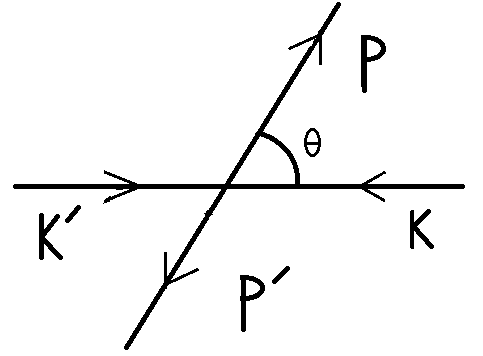
\includegraphics[scale=0.3]{kinematics.png}\\
\textbf{Figure:} Scattering diagram of $2 \longrightarrow 2$ process
\end{center}

Two incoming DM particles with four momenta $k_\mu$ and $k\prime_\mu$ will annihilate and outgoing particles are with $p$ and $p\prime$. $3-momentum\; \vec{p}$ make an angle $\theta$ with the incoming particles line. As the mass of the incoming particles is the same, and we are in the center of the mass frame, let the energy of each particle be $\omega$. Let the mass of the DM be $m_\chi$. We will put non-relativistic limit: $\mid \vec{k} \mid \approx m_\chi v$
 .Therefore:

Let the magnitude of the 3-momentum of the incoming particles be $k$ and the magnitude of the outgoing particles be $p_f$. These scattering processes are two-dimensional cases. Realizing all these, we can write:


\begin{align*}
&k^\mu=(\omega,k,0,0)\\
&k\prime^\mu =(\omega,-k,0,0)\\
&p^\mu =(\omega,p_f \cos\theta, p_f \sin\theta,0)\\
&p\prime^\mu =(\omega,-p_f \cos\theta, -p_f \sin\theta,0)
\end{align*}

Now we get:

\begin{align*}
&k^\mu k\prime_\mu = \omega^2+k^2\\
&k^\mu p_\mu = \omega^2-kp_f \cos\theta\\
&k^\mu p\prime_\mu = \omega^2 + kp_f \cos\theta\\
&k\prime^\mu p_\mu = \omega^2 + kp_f \cos\theta\\
&k\prime^\mu p\prime\mu = \omega^2-kp_f \cos\theta\\
&p^\mu p\prime_\mu =\omega^2+p_f^2
\end{align*}\\
and
\begin{eqnarray}
&\omega = \sqrt{(\mid \vec{k} \mid)^2 + m_\chi^2}\\
&\Rightarrow \omega^2 =(\mid \vec{k} \mid)^2 + m_\chi^2\\
&\Rightarrow \omega^2 \approx m_\chi^2 v^2 + m_\chi^2\\
&\Rightarrow \omega^2 \approx m_\chi^2 (1+v^2)\\
&\Rightarrow \omega \approx m_\chi \sqrt{(1+v^2)}\\
&\Rightarrow \omega \approx m_\chi (1+\frac{v^2}{2})
\end{eqnarray}

For these processes, product particles have the same mass. Therefore conservation of energy implies that each of them has the same energy $\omega$.


\begin{eqnarray}
&\omega^2 = (\mid \vec{p} \mid)^2 + m^2 \\
& \Rightarrow \omega^2 = p_f^2+ m^2\\
&\Rightarrow p_f^2= \omega^2 - m^2 \\
& \Rightarrow p_f \approx \sqrt{m_\chi^2 v^2 + m_\chi^2 -m^2}
\end{eqnarray}

To compute cross-section we will be using the following equation:

\begin{align}
\frac{d\sigma}{d\Omega}= \frac{1}{64 \pi^2 s} \frac{p_f}{k} |\mathcal{M}|^2 \label{cross}
\end{align}

In the case of unpolarized final states, we have to average over the polarization states.


For a detailed derivation of this formula one can look into \cite{pes}


\subsection{DM DM$\longrightarrow q \bar{q}$}
 Effective operator, $\mathscr{L}_{eff} : \frac{c}{\Lambda} \phi^2 \bar{q}q$
\begin{center}
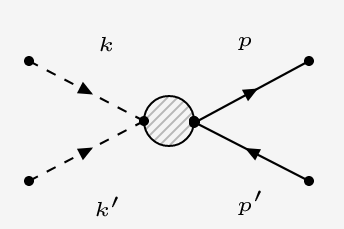
\includegraphics[scale=0.5]{qqbar.png}
\end{center}


Probability amplitude:
\begin{align*}
& i \mathcal{M}= \frac{c}{\Lambda} \bar{u}^s_q(p)v^{s\prime}_q(p\prime)\\
&\Rightarrow -i \mathcal{M} = \frac{c}{\Lambda} \bar{v}_q^{s\prime}(p\prime) u^s_q(p)
\end{align*}

Therefore we get:

\begin{align*}
&\frac{1}{2} \sum_s \sum_{s\prime} (|\mathcal{M}|)^2 = \frac{c^2}{\Lambda^2} \frac{1}{2} Tr \{ ( \slashed{p}\prime-m_q)(\slashed{p}+m_q) \} \\
&=  \frac{c^2}{\Lambda^2} \frac{1}{2} Tr\{(\gamma^\mu p\prime_\mu -m_q)(\gamma^\nu p_\nu +m_q)  \}\\
&= \frac{2c^2}{\Lambda^2} (p^\mu p\prime_\mu-m_q^2)\\
&=\frac{2c^2}{\Lambda^2} (\omega^2+ p_f^2 -m_q^2)\\
&= \frac{4c^2}{\Lambda^2} p_f^2 
\end{align*}\\
Using \ref{cross} we get,
\begin{align*}
&\frac{d\sigma}{d\Omega}= \frac{1}{64 \pi^2 s} \frac{p_f}{k} \frac{1}{2} \sum_s \sum_{s\prime} (|\mathcal{M}|)^2\\
&\Rightarrow \frac{d\sigma}{d\Omega}=\frac{1}{64 \pi^2 s} \frac{p_f}{k} \frac{4c^2}{\Lambda^2} p_f^2\\
&\Rightarrow \frac{d\sigma}{d\Omega}= \frac{1}{16 \pi^2} \frac{c^2}{\Lambda^2} \frac{1}{s} \frac{p_f^3}{k}\\
&\Rightarrow \sigma = \frac{c^2}{4 \pi \Lambda^2} \frac{1}{4 \omega^2} \frac{p_f^3}{k}\\
&\Rightarrow \sigma =\frac{1}{16 \pi} \frac{c^2}{\Lambda^2} \frac{1}{m_\chi v} \omega (1-\frac{m_q^2}{\omega^2})^{3/2}\\
&\Rightarrow \sigma v \approx \frac{1}{16 \pi} \frac{c^2}{\Lambda^2} \frac{1}{m_\chi} m_\chi(1+\frac{v^2}{2}) \{1-\frac{m_q^2}{m_\chi^2(1+v^2)} \}^{3/2}\\
&\Rightarrow \sigma v \approx \frac{1}{16 \pi} \frac{c^2}{\Lambda^2} (1+\frac{v^2}{2}) \{1-\frac{m_q^2}{m_\chi^2}(1+v^2)^{-1} \}^{3/2}\\
&\Rightarrow <\sigma v> \approx \frac{1}{16 \pi} \frac{c^2}{\Lambda^2} (1+\frac{v^2}{2}) \{1-\frac{m_q^2}{m_\chi^2}(1-v^2) \}^{3/2}\\
&\Rightarrow <\sigma v> \approx \frac{1}{16 \pi} \frac{c^2}{\Lambda^2} (1+\frac{v^2}{2}) \{1-\frac{m_q^2}{m_\chi^2} + \frac{m_q^2}{m_\chi} v^2 \}^{3/2}\\
&\approx \frac{1}{16 \pi} \frac{c^2}{\Lambda^2} (1+\frac{v^2}{2}) (1-\frac{m_q^2}{m_\chi^2})^{3/2} (1+\frac{m_q^2}{m_\chi^2-m_q^2} v^2)^{3/2}\\
& \approx \frac{1}{16 \pi} \frac{c^2}{\Lambda^2} (1+\frac{v^2}{2}) (1-\frac{m_q^2}{m_\chi^2})^{3/2} (1+ \frac{3}{2} \frac{m_q^2}{m_\chi^2-m_q^2}v^2)\\
& \approx \frac{1}{16 \pi} \frac{c^2}{\Lambda^2} (1-\frac{m_q^2}{m_\chi^2})^{3/2} 
\left(1+ \frac{m_\chi^2 +2m_q^2}{m_\chi^2-m_q^2} \frac{v^2}{2}\right)
\end{align*}

Thus, 

\begin{equation}
<\sigma v > \approx \frac{1}{16 \pi} \frac{c^2}{\Lambda^2} (1-\frac{m_q^2}{m_\chi^2})^{3/2} 
\left(1+ \frac{m_\chi^2 +2m_q^2}{m_\chi^2-m_q^2} \frac{v^2}{2}\right) \label{qqcross}
\end{equation}

\newpage

\subsection{DM DM $\longrightarrow W^+W^-$}

Cross-section: To compute cross-section for this case we use the following Feynman diagram and vertex factor \ref{wv}.

\begin{center}
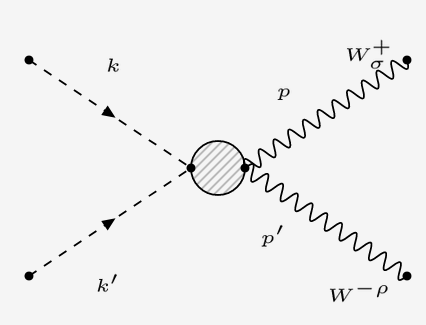
\includegraphics[scale=0.5]{WW.png}
\end{center}


\begin{align*}
&i \mathcal{M}= \epsilon^{(\lambda)}_\sigma (p) \frac{16c_1}{\Lambda^2} \{(p\cdot p^\prime) g_\rho^{\;\sigma}-p^{\prime \sigma} p_\rho\} \epsilon^{* (\lambda^\prime) \rho}(p^\prime)\\
&-i \mathcal{M}^* = \frac{16c_1}{\Lambda^2} \epsilon^{(\lambda^\prime) \mu}(p^\prime) \{(p\cdot p^\prime) g^{\;\nu}_\mu -p^{\prime \nu} p_\mu \} \epsilon^{*(\lambda)}_\nu (p)
\end{align*}

Considering polarization states and averaging,
\begin{align*}
& \frac{1}{3} \sum_\lambda \sum_{\lambda^\prime} |\mathcal{M}|^2  = \frac{256 c^2_1}{3\Lambda^4} \left\{-g^{\mu \rho} + \frac{p^{\prime \mu} p^{\prime \rho}}{m^2_z} \right\}\{(p\cdot p^\prime) g_\rho^{\;\sigma}-p^{\prime \sigma} p_\rho\} \\
&\;\;\;\; \left\{ -g_{\sigma \nu} +\frac{p_\sigma p_\nu}{m^2_z} \right\} \{(p\cdot p^\prime) g^{\;\nu}_\mu -p^{\prime \nu} p_\mu \}\\
& =\frac{256 c^2_1}{3\Lambda^4} \left\{-(p \cdot p^\prime) g^{\mu \sigma} +p^{\prime \sigma} p^{\mu} +(p \cdot p^\prime) \frac{p^{\prime \sigma} p^{\prime \mu}}{m^2_w} -(p\cdot p^\prime) \frac{p^{\prime \mu} p^{\prime \sigma}}{m^2_w} \right\}\\
& \;\;\;\; \left\{-(p \cdot p^\prime) g_{\mu \sigma}+p^\prime_\sigma p_\mu +(p \cdot p^\prime) \frac{p_\sigma p_\mu}{m^2_w} -(p \cdot p^\prime) \frac{p_\sigma p_\mu}{m^2_w}   \right\} \\
&=\frac{256 c^2_1}{3\Lambda^4} \left\{-(p \cdot p^\prime) g^{\mu \sigma} + p^{\prime \sigma} p^\mu \right\} \left\{-(p \cdot p^\prime) g_{\mu \sigma} + p^\prime_\sigma p_\mu \right\}\\
& =\frac{256 c^2_1}{3\Lambda^4}  \{ 4(p \cdot p^\prime)^2 - (p \cdot p^\prime)^2 -(p \cdot p^\prime)^2 + (p^\prime \cdot p^\prime) (p \cdot p)  \} \\
&  =\frac{256 c^2_1}{3\Lambda^4} \{ 2(p \cdot p^\prime)^2 +m_w^4\}
\end{align*}
Using \ref{cross}, cross section for $2 \longrightarrow 2$ process:
\begin{align*}
\frac{d \sigma}{d \Omega} & = \frac{1}{64 \pi^2 s} \frac{p_f}{k} \frac{1}{2} \sum_\lambda \sum_{\lambda^\prime} |\mathcal{M}|^2 \\
&=\frac{1}{64 \pi^2 s} \frac{p_f}{k}  \frac{256 c^2_1}{3\Lambda^4} \{ 2(p \cdot p^\prime)^2 +m_w^4\}\\
&= \frac{4 c^2_1}{3\Lambda^4 \pi^2} \frac{p_f}{4 \omega^2 k} \{ 2 (\omega^2 +p_f^2)^2 +m_w^4 \} \\
&\approx \frac{4c^2_1}{3 \pi^2 \Lambda^4}  \frac{1}{m_\chi v} \frac{\sqrt{\omega^2 -m^2_w}}{\omega^2} \{ 2(2 \omega^2 -m_w^2 )^2 +m_w^4 \} \\
&\approx \frac{c^2_1}{3 \pi^2 \Lambda^4}  \frac{1}{m_\chi v} \sqrt{1-\frac{m^2_w}{\omega^2}} \; \omega^{-1}  \{ 2(2k^2 + 2 m^2_\chi -m^2_w)^2 +m^4_w \}\\
&\approx \frac{c^2_1}{3 \pi^2 \Lambda^4}  \frac{1}{m_\chi v} \sqrt{1-\frac{m^2_w}{\omega^2}} \; (m^2_\chi v^2 + m^2_\chi )^{- 1/2} \left\{  2 (2m^2_\chi - m^2_w)^2 \right. \\
&\;\;\;\;\;\;\;\; \left. \left( 1+ \frac{2m^2_\chi}{2m^2_\chi - m^2_w} v^2 \right)^2 +m^4_w \right\} \\
&\approx \frac{c^2_1}{3 \pi^2 \Lambda^4}  \frac{1}{m_\chi v} \sqrt{1-\frac{m^2_w}{m^2_\chi}+\frac{m^2_w}{m^2_\chi}v^2}\; \; \frac{1}{m_\chi} \left(1-\frac{v^2}{2}\right) \left\{  2 (2m^2_\chi - m^2_w)^2 \right. \\
& \;\;\;\;\;\;\;\; \left. \left( 1+ \frac{4m^2_\chi}{2m^2_\chi - m^2_w} v^2 \right) +m^4_w \right\} \\
&\approx \frac{c^2_1}{3 \pi^2 \Lambda^4}  \frac{1}{m_\chi^2 v} \sqrt{1-\frac{m^2_w}{m^2_\chi}} \sqrt{1+\frac{m^2_w}{m^2_\chi - m^2_w} v^2}\; \left(1-\frac{v^2}{2}\right) \\
& \;\;\;\;\;\; \;\;\;\;\;\;\;\;\;\; \{ m^4_w + 2(2 m^2_\chi - m^2_w)^2 + 4m^2_\chi (2m^2_\chi -m^2_w) v^2 \}\\
&\approx \frac{c^2_1}{3 \pi^2 \Lambda^4}  \frac{1}{m^2_\chi v} \sqrt{1-\frac{m^2_w}{m^2_\chi}} \left\{ 1+\frac{m^2_w}{2(m^2_\chi-m^2_w)} v^2 \right\} \{ m^4_w + 2(2m^2_\chi - m^2_w)^2 \\
& \;\;\;\;\; - \frac{m^4_w v^2}{2} + (2 m^2_\chi - m^2_w)^2 v^2 + 4 m^2_\chi ( 2 m^2_\chi - m^2_w )^2 v^2\} \\
&\approx  \frac{c^2_1}{3 \pi^2 \Lambda^4}  \frac{1}{m^2_\chi v}  \sqrt{1-\frac{m^2_w}{m^2_\chi}} \left[ m^4_w + 2(2 m^2_\chi -m^2_w)^2 + \right. \\
& \left. \left\{ \frac{ m^6_w+2 m^2_w (2 m^2_\chi - m^2_w)^2 }{2(m^2_\chi - m^2_w)} -\frac{m^4_w}{2} + (2 m^2_\chi - m^2_w) + 4 m^2_\chi (2 m^2_\chi - m^2_w)^2 \right\} v^2 \right]
\end{align*}


Therefore the cross-section:

\begin{align*}
&\sigma  \approx \frac{4c^2_1}{3\pi \Lambda^4}  \frac{1}{m^2_\chi v}  \sqrt{1-\frac{m^2_w}{m^2_\chi}} \left[ m^4_w + 2(2 m^2_\chi -m^2_w)^2 + \right. \\
& \left. \left\{ \frac{ m^6_w+2 m^2_w (2 m^2_\chi - m^2_w)^2 }{2(m^2_\chi - m^2_w)} -\frac{m^4_w}{2} + (2 m^2_\chi - m^2_w) + 4 m^2_\chi (2 m^2_\chi - m^2_w)^2 \right\} v^2  \right]\\
&\Rightarrow <\sigma v> \approx \frac{4c^2_1}{3 \pi \Lambda^4}  \frac{1}{m^2_\chi}  \sqrt{1-\frac{m^2_w}{m^2_\chi}} \left[ m^4_w + 2(2 m^2_\chi -m^2_w)^2 + \right. \\
& \left. \left\{ \frac{ m^6_w+2 m^2_w (2 m^2_\chi - m^2_w)^2 }{2(m^2_\chi - m^2_w)} -\frac{m^4_w}{2} + (2 m^2_\chi - m^2_w) + 4 m^2_\chi (2 m^2_\chi - m^2_w)^2 \right\} v^2  \right]  
\end{align*}

Finally, we get:

\begin{multline}
<\sigma v> \approx \frac{4c^2_1}{3 \pi \Lambda^4}  \frac{1}{m^2_\chi}  \sqrt{1-\frac{m^2_w}{m^2_\chi}} \left[ m^4_w + 2(2 m^2_\chi -m^2_w)^2 + \right. \\
\left. \left\{ \frac{ m^6_w+2 m^2_w (2 m^2_\chi - m^2_w)^2 }{2(m^2_\chi - m^2_w)} -\frac{m^4_w}{2} + (2 m^2_\chi - m^2_w) + 4 m^2_\chi (2 m^2_\chi - m^2_w)^2 \right\} v^2  \right]  \label{wwcross} 
\end{multline}

\newpage

\subsection{DM DM $\longrightarrow ZZ$}


Cross-section: To compute cross-section for this case we use the following Feynman diagram and vertex factor \ref{zv}.

\begin{center}
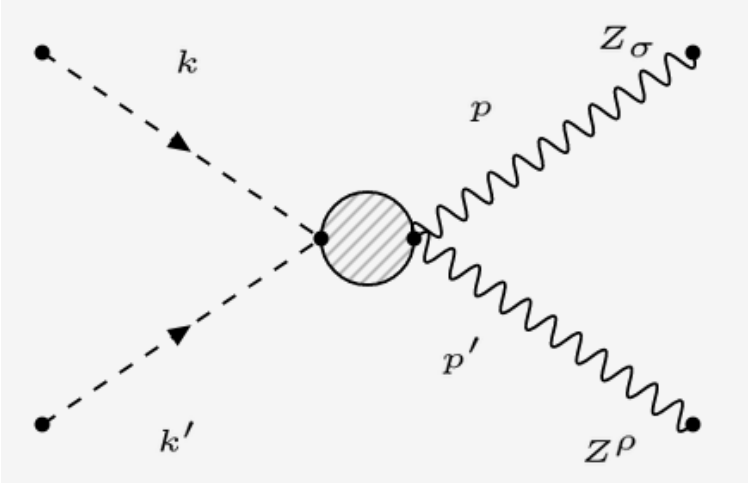
\includegraphics[scale=0.3]{ZZ.png}
\end{center}



\begin{align*}
&i \mathcal{M}=- \epsilon^{(\lambda)}_\sigma (p) \frac{8c^\prime}{\Lambda^2} \{(p\cdot p^\prime) g_\rho^{\;\sigma}-p^{\prime \sigma} p_\rho\} \epsilon^{ (\lambda^\prime) \rho}(p^\prime)\\
&-i \mathcal{M}^* = - \frac{8c^\prime}{\Lambda^2} \epsilon^{*(\lambda^\prime) \mu}(p^\prime) \{(p\cdot p^\prime) g^{\;\nu}_\mu -p^{\prime \nu} p_\mu \} \epsilon^{*(\lambda)}_\nu (p)
\end{align*}

Considering polarization states and averaging,
\begin{align*}
& \frac{1}{3} \sum_\lambda \sum_{\lambda^\prime} |\mathcal{M}|^2  = \frac{64 c^2_1}{3\Lambda^4} \left\{-g^{\mu \rho} + \frac{p^{\prime \mu} p^{\prime \rho}}{m^2_z} \right\}\{(p\cdot p^\prime) g_\rho^{\;\sigma}-p^{\prime \sigma} p_\rho\}\\ 
&\;\;\;\;\;\;\;\;\;\; \left\{ -g_{\sigma \nu} +\frac{p_\sigma p_\nu}{m^2_z} \right\} \{(p\cdot p^\prime) g^{\;\nu}_\mu -p^{\prime \nu} p_\mu \}\\
& =\frac{64 c^{\prime2}}{3\Lambda^4} \left\{-(p \cdot p^\prime) g^{\mu \sigma} +p^{\prime \sigma} p^{\mu} +(p \cdot p^\prime) \frac{p^{\prime \sigma} p^{\prime \mu}}{m^2_z} -(p\cdot p^\prime) \frac{p^{\prime \mu} p^{\prime \sigma}}{m^2_z} \right\}\\
& \;\;\;\; \left\{-(p \cdot p^\prime) g_{\mu \sigma}+p^\prime_\sigma p_\mu +(p \cdot p^\prime) \frac{p_\sigma p_\mu}{m^2_z} -(p \cdot p^\prime) \frac{p_\sigma p_\mu}{m^2_z}   \right\} \\
&=\frac{64 c^{\prime 2}}{3\Lambda^4} \left\{-(p \cdot p^\prime) g^{\mu \sigma} + p^{\prime \sigma} p^\mu \right\} \left\{-(p \cdot p^\prime) g_{\mu \sigma} + p^\prime_\sigma p_\mu \right\}\\
& =\frac{64 c^{\prime 2}}{3\Lambda^4}  \{ 4(p \cdot p^\prime)^2 - (p \cdot p^\prime)^2 -(p \cdot p^\prime)^2 + (p^\prime \cdot p^\prime) (p \cdot p)  \} \\
&  =\frac{64 c^{\prime 2}}{3\Lambda^4} \{ 2(p \cdot p^\prime)^2 +m_z^4\}
\end{align*}
We have to divide this with a combinatorial factor of $2$ due to $Z$-bosons. Using \ref{cross}, cross section for $2 \longrightarrow 2$ process:
\begin{align*}
\frac{d \sigma}{d \Omega} & = \frac{1}{64 \pi^2 s} \frac{p_f}{k} \frac{1}{4} \sum_\lambda \sum_{\lambda^\prime} |\mathcal{M}|^2 \\
&=\frac{1}{64 \pi^2 s} \frac{p_f}{k}  \frac{64 c^{\prime 2}}{6\Lambda^4} \{ 2(p \cdot p^\prime)^2 +m_z^4\}\\
&= \frac{2c^{\prime 2}}{3\Lambda^4 \pi^2} \frac{p_f}{4 \omega^2 k} \{ 2 (\omega^2 +p_f^2)^2 +m_z^4 \} \\
&\approx \frac{c^{\prime 2}}{24 \pi^2 \Lambda^4}  \frac{1}{m_\chi v} \frac{\sqrt{\omega^2 -m^2_z}}{\omega^2} \{ 2(2 \omega^2 -m_z^2 )^2 +m_z^4 \} \\
&\approx \frac{c^{\prime 2}}{24 \pi^2 \Lambda^4}  \frac{1}{m_\chi v} \sqrt{1-\frac{m^2_z}{\omega^2}} \; \omega^{-1}  \{ 2(2k^2 + 2 m^2_\chi -m^2_z)^2 +m^4_z \}\\
&\approx \frac{c^{\prime 2}}{24 \pi^2 \Lambda^4}  \frac{1}{m_\chi v} \sqrt{1-\frac{m^2_z}{\omega^2}} \; (m^2_\chi v^2 + m^2_\chi )^{- 1/2} \left\{  2 (2m^2_\chi - m^2_z)^2 \right. \\
& \;\;\;\;\;\;\;\; \left. \left( 1+ \frac{2m^2_\chi}{2m^2_\chi - m^2_z} v^2 \right)^2 +m^4_z \right\} \\
&\approx\frac{c^{\prime 2}}{24 \pi^2 \Lambda^4}  \frac{1}{m_\chi v} \sqrt{1-\frac{m^2_z}{m^2_\chi}+\frac{m^2_z}{m^2_\chi}v^2}\; \; \frac{1}{m_\chi} \left(1-\frac{v^2}{2}\right) \left\{  2 (2m^2_\chi - m^2_z)^2 \right.\\
&\;\;\;\;\;\;\;\; \;\left. \left( 1+ \frac{4m^2_\chi}{2m^2_\chi - m^2_z} v^2 \right) +m^4_z \right\} \\
&\approx \frac{c^{\prime 2}}{24 \pi^2 \Lambda^4} \frac{1}{m_\chi^2 v} \sqrt{1-\frac{m^2_z}{m^2_\chi}} \sqrt{1+\frac{m^2_z}{m^2_\chi - m^2_z} v^2}\; \left(1-\frac{v^2}{2}\right) \\
& \;\;\;\;\;\; \;\;\;\;\;\;\;\;\;\; \left\{ m^4_z + 2(2 m^2_\chi - m^2_z)^2 + 4m^2_\chi (2m^2_\chi -m^2_z) v^2 \right\}\\
&\approx \frac{c^{\prime 2}}{24 \pi^2 \Lambda^4}  \frac{1}{m^2_\chi v} \sqrt{1-\frac{m^2_z}{m^2_\chi}} \left\{ 1+\frac{m^2_z}{2(m^2_\chi-m^2_z)} v^2 \right\} \left\{ m^4_z + 2(2m^2_\chi - m^2_z)^2 \right.\\
& \;\;\;\;\; \left. - \frac{m^4_z v^2}{2} + (2 m^2_\chi - m^2_z)^2 v^2 + 4 m^2_\chi ( 2 m^2_\chi - m^2_z )^2 v^2 \right\} \\
&\approx  \frac{c^{\prime 2}}{24 \pi^2 \Lambda^4}  \frac{1}{m^2_\chi v}  \sqrt{1-\frac{m^2_z}{m^2_\chi}} \left[ m^4_z + 2(2 m^2_\chi -m^2_z)^2 + \right. \\
& \left. \left\{ \frac{ m^6_z+2 m^2_z (2 m^2_\chi - m^2_z)^2 }{2(m^2_\chi - m^2_z)} -\frac{m^4_z}{2} + (2 m^2_\chi - m^2_z) + 4 m^2_\chi (2 m^2_\chi - m^2_z)^2 \right\} v^2  \right]
\end{align*}


Therefore the cross-section:

\begin{align*}
&\sigma  \approx \frac{4c^2_1}{3\pi \Lambda^4}  \frac{1}{m^2_\chi v}  \sqrt{1-\frac{m^2_z}{m^2_\chi}} \left[ m^4_z + 2(2 m^2_\chi -m^2_z)^2 + \right.\\
& \left. \left\{ \frac{ m^6_z+2 m^2_z (2 m^2_\chi - m^2_z)^2 }{2(m^2_\chi - m^2_z)} -\frac{m^4_z}{2} + (2 m^2_\chi - m^2_z) + 4 m^2_\chi (2 m^2_\chi - m^2_z)^2 \right\} v^2  \right]\\
&\Rightarrow <\sigma v> \approx \frac{4c^2_1}{3 \pi \Lambda^4}  \frac{1}{m^2_\chi}  \sqrt{1-\frac{m^2_z}{m^2_\chi}} \left[ m^4_z + 2(2 m^2_\chi -m^2_z)^2 + \right.\\
& \left. \left\{ \frac{ m^6_z+2 m^2_z (2 m^2_\chi - m^2_z)^2 }{2(m^2_\chi - m^2_z)} -\frac{m^4_z}{2} + (2 m^2_\chi - m^2_z) + 4 m^2_\chi (2 m^2_\chi - m^2_z)^2 \right\} v^2  \right]  
\end{align*}

Finally, the cross-section we get:

\begin{multline}
<\sigma v> \approx \frac{4c^2_1}{3 \pi \Lambda^4}  \frac{1}{m^2_\chi}  \sqrt{1-\frac{m^2_z}{m^2_\chi}} \left[ m^4_z + 2(2 m^2_\chi -m^2_z)^2 + \right.\\
\left. \left\{ \frac{ m^6_z+2 m^2_z (2 m^2_\chi - m^2_z)^2 }{2(m^2_\chi - m^2_z)} -\frac{m^4_z}{2} + (2 m^2_\chi - m^2_z) + 4 m^2_\chi (2 m^2_\chi - m^2_z)^2 \right\} v^2  \right] \label{zzcross}  
\end{multline}


\newpage


\subsection{DM DM $\longrightarrow \gamma \gamma$}

Cross-section: To compute cross-section for this case we use the following Feynman diagram and vertex factor \ref{gv}.

\begin{center}
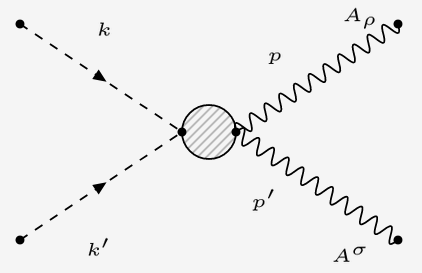
\includegraphics[scale=0.5]{GG.png}
\end{center}

\begin{align*}
&i \mathcal{M} = -\epsilon^{(r)}_\rho(p) \frac{8c_0}{\Lambda^2} \left\{ (p\cdot p^\prime) g^\rho_{\; \sigma }- p^{\prime \rho} p_\sigma \right\} \epsilon^{(r^\prime)\sigma} (p^\prime)\\
& -i \mathcal{M}^* = -\epsilon^{*(r^\prime) \mu} (p^\prime) \frac{8c_0}{\Lambda^2} \left\{ (p\cdot p^\prime) g^\nu_{\; \mu }- p^{\prime \nu} p_\mu \right\} \epsilon^{*(r)}_\nu (p)\\
&\therefore \frac{1}{2} \sum_r \sum_{r^\prime} |\mathcal{M}|^2 = \frac{64 c^2_0}{\Lambda^4} (p \cdot p^\prime)^2
\end{align*}

Now the differential cross-section \ref{cross}:

\begin{align*}
\frac{d\sigma}{d\Omega} &= \frac{1}{64 \pi^2 s}\frac{1}{2} \sum_r \sum_{r^\prime} |\mathcal{M}|^2  \frac{p_f}{k}\\
&= \frac{1}{64 \pi^2 s}  \frac{64 c^2_0}{\Lambda^4} (p \cdot p^\prime)^2 \frac{p_f}{k}
\end{align*}


Therefore,
\begin{align}
<\sigma v> = \frac{4}{\pi} \frac{c^2_0}{\Lambda^4} m^2_\chi \left(1+\frac{3}{2} v^2 \right) \label{ggcross}
\end{align}



\subsection{DM DM $\longrightarrow \gamma Z$}




Before we compute the cross-section for this annihilation process, we need to evaluate the dynamic parameters as the product particles have different masses.\\

Let $\omega$ be the energy of each DM particle.  Let the magnitude of the 3-momentum of the incoming particles be $k$ and the magnitude of the outgoing particles be $p_f$. These scattering processes are two-dimensional cases. Realizing all these, we can write:


\begin{align*}
&k^\mu=(\omega,k,0,0)\\
&k\prime^\mu =(\omega,-k,0,0)\\
&p^\mu =(E_z,p_f \cos\theta, p_f \sin\theta,0)\\
&p\prime^\mu =(p_f,-p_f \cos\theta, -p_f \sin\theta,0)
\end{align*}

Now we get:

\begin{align*}
&k^\mu k^\prime_\mu = \omega^2+k^2\\
&k^\mu p_\mu = E_z \omega-kp_f \cos\theta\\
&k^\mu p^\prime_\mu = \omega p_f + kp_f \cos\theta\\
&k^\prime_\mu p^\mu = E_z \omega + kp_f \cos\theta\\
&k^{\prime\mu} p^\prime_\mu =  \omega p_f -kp_f \cos\theta\\
&p^\mu p^\prime_\mu = p_f E_z+p_f^2
\end{align*}


For this case, we will recall the relations involving DM particles: 
\begin{eqnarray}
&\omega = \sqrt{(\mid \vec{k} \mid)^2 + m_\chi^2}\\
&\Rightarrow \omega^2 =(\mid \vec{k} \mid)^2 + m_\chi^2\\
&\Rightarrow \omega^2 \approx m_\chi^2 v^2 + m_\chi^2\\
&\Rightarrow \omega^2 \approx m_\chi^2 (1+v^2)\\
&\Rightarrow \omega \approx m_\chi \sqrt{(1+v^2)}\\
&\Rightarrow \omega \approx m_\chi (1+\frac{v^2}{2})
\end{eqnarray}
From the Conservation of momentum, we can deduce that $\gamma$ and $Z$ both have an equal magnitude of momentum $p_f$. Now, let's apply the conservation of energy:
\begin{align}
& 2 \omega = E_\gamma+ E_z\\
&\Rightarrow 2 \omega = p_f+ \sqrt{p^2_f+ m^2_z}\\
&\Rightarrow 4 \omega^2 -4 \omega p_f + p^2_f = p^2_f +m^2_z\\
& \therefore p_f= \frac{4\omega^2 - m^2_z}{4 \omega}
\end{align}




\newpage



Cross section:Cross-section: To compute cross-section for this case we use the following Feynman diagram and vertex factor \ref{gzv}.

\begin{center}
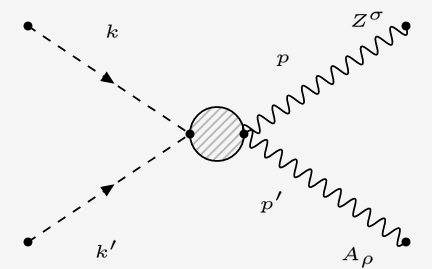
\includegraphics[scale=0.5]{GW.png}
\end{center}

\begin{align*}
&i \mathcal{M} = \tilde{a}^{(\lambda^\prime)}_\rho(p^\prime) \left[-\frac{8\tilde{c}}{\Lambda^2} \{ (p.p^\prime) g^\rho_{\; \sigma} - p^{\prime \rho} p_\sigma \} \right] \tilde{z}^{(\lambda) \sigma}(p)\\
&-i \mathcal{M}^* = \tilde{z}^{*(\lambda) \mu}(p) \left[ -\frac{8\tilde{c}}{\Lambda^2} \{ (p.p^\prime) g^\nu_{\; \mu} - p^{\prime \nu} p_\mu \} \right] \tilde{a}^{*(\lambda^\prime)}_\nu(p^\prime)\\
& \therefore \frac{1}{2} \sum_\lambda \sum_{\lambda^\prime} |\mathcal{M}|^2 = \frac{64 \tilde{c}^2}{\lambda^4} (p \cdot p^\prime)^2
\end{align*}


Now, the differential cross-section from \ref{cross}:

\begin{align*}
\frac{d\sigma}{d\Omega} &= \frac{1}{64 \pi^2 s} \frac{p_f}{k} \frac{1}{2} \sum_\lambda \sum_{\lambda^\prime} |\mathcal{M}|^2\\
&= \frac{1}{64 \pi^2 s} \frac{p_f}{k} \frac{64 \tilde{c}^2}{\lambda^4} (p \cdot p^\prime)^2\\
&= \frac{1}{4 \pi^2} \frac{\tilde{c}^2}{\Lambda^4} \frac{1}{k} \frac{p^3_f}{\omega^2}(E_z + p_f)^2 \\
\therefore \sigma &= \frac{1}{\pi} \frac{\tilde{c}^2}{\Lambda^4} \frac{1}{k} \frac{p^3_f}{\omega^2}(E_z + p_f)^2 \\
\therefore <\sigma v> &\approx \frac{1}{\pi} \frac{\tilde{c}^2}{\Lambda^4} m^2_\chi \left( 1- \frac{m^2_z}{4 m^2_\chi} \right)^3 \left\{1 + \frac{4m^2_\chi - 3m^2_z}{(4m^2_\chi - m^2_z)} v^2\right\}
\end{align*}


Thus,

\begin{equation}
 <\sigma v> \approx \frac{1}{\pi} \frac{\tilde{c}^2}{\Lambda^4} m^2_\chi \left( 1- \frac{m^2_z}{4 m^2_\chi} \right)^3 \left\{1 + \frac{4m^2_\chi - 3m^2_z}{(4m^2_\chi - m^2_z)} v^2\right\} \label{gzcross}
\end{equation}

\pagebreak

\chapter{Result and Discussion} 
 In this thesis paper, our dark matter candidate was a standard model singlet. Our interested annihilation process was $ DM\;DM \longrightarrow q \bar{q}\; (from\; \mathcal{O}_1),\\ \; \; DM\; DM \longrightarrow W^+W^-(From\; \mathcal{O}_2), \; \;
DM\; DM \longrightarrow ZZ (from\; \mathcal{O}_2 \; and\; \mathcal{O}_3 ),\\ \; \; DM\; DM \longrightarrow \gamma Z (from\; \mathcal{O}_2 \; and\; \mathcal{O}_3 ) , \; \; DM\; DM \longrightarrow \gamma  \gamma (from\; \mathcal{O}_2  \; and\; \mathcal{O}_3 )$.  We constructed our effective operators such that it is standard model invariant. We set a cut-off $\Lambda$ and coupling constants for different operators.
 
 
 We recall the effective operators we constructed in section 4.2, again we write them in a table:
 
 \begin{center}
\begin{tabular}{|c|c|}
\hline
Label & Operators\\ \hline
$\mathcal{O}_1$ & $\frac{c}{\Lambda} \phi^2 \bar{q}q$\\ \hline
$\mathcal{O}_2$ & $\frac{c_1}{\Lambda^2} \phi^2 W_{\mu \nu a} W^{\mu \nu}_a$ \\ \hline

$\mathcal{O}_3$ & $\frac{c_2}{\Lambda^2} \phi^2 B_{\mu \nu} B^{\mu \nu}$\\ \hline
\end{tabular}
\end{center}

We computed the cross-section times velocity for $ DM\;DM \longrightarrow q \bar{q}\; (from\; \mathcal{O}_1),\\ \; \; DM\; DM \longrightarrow W^+W^-(From\; \mathcal{O}_2), \; \;
DM\; DM \longrightarrow ZZ (from\; \mathcal{O}_2 \; and\; \mathcal{O}_3 ),\\ \; \; DM\; DM \longrightarrow \gamma Z (from\; \mathcal{O}_2 \; and\; \mathcal{O}_3 ) , \; \; DM\; DM \longrightarrow \gamma  \gamma (from\; \mathcal{O}_2  \; and\; \mathcal{O}_3 )$. 


\section{Result}

The cross sections we computed, equation (\ref{qqcross}) , (\ref{wwcross}) , (\ref{zzcross}) , (\ref{ggcross}) ,(\ref{gzcross}):






q-channel:
\begin{align}
<\sigma v > \approx \frac{1}{16 \pi} \frac{c^2}{\Lambda^2} (1-\frac{m_q^2}{m_\chi^2})^{3/2} 
\left(1+ \frac{m_\chi^2 +2m_q^2}{m_\chi^2-m_q^2} \frac{v^2}{2}\right)
\end{align}\\

W-channel:
\begin{multline}
<\sigma v> \approx \frac{4c^2_1}{3 \pi \Lambda^4}  \frac{1}{m^2_\chi}  \sqrt{1-\frac{m^2_w}{m^2_\chi}} \left[ m^4_w + 2(2 m^2_\chi -m^2_w)^2 + \right. \\
\left. \left\{ \frac{ m^6_w+2 m^2_w (2 m^2_\chi - m^2_w)^2 }{2(m^2_\chi - m^2_w)} -\frac{m^4_w}{2} + (2 m^2_\chi - m^2_w) + 4 m^2_\chi (2 m^2_\chi - m^2_w)^2 \right\} v^2  \right] 
\end{multline}\\

Z-channel:
\begin{multline}
<\sigma v> \approx \frac{4c^2_1}{3 \pi \Lambda^4}  \frac{1}{m^2_\chi}  \sqrt{1-\frac{m^2_z}{m^2_\chi}} \left[ m^4_z + 2(2 m^2_\chi -m^2_z)^2 + \right.\\
\left. \left\{ \frac{ m^6_z+2 m^2_z (2 m^2_\chi - m^2_z)^2 }{2(m^2_\chi - m^2_z)} -\frac{m^4_z}{2} + (2 m^2_\chi - m^2_z) + 4 m^2_\chi (2 m^2_\chi - m^2_z)^2 \right\} v^2  \right]
\end{multline}\\



$\gamma$-channel:

\begin{align}
<\sigma v> = \frac{4}{\pi} \frac{c^2_0}{\Lambda^4} m^2_\chi \left(1+\frac{3}{2} v^2 \right)
\end{align}\\

$\gamma$Z-channel:
\begin{equation}
 <\sigma v> \approx \frac{1}{\pi} \frac{\tilde{c}^2}{\Lambda^4} m^2_\chi \left( 1- \frac{m^2_z}{4 m^2_\chi} \right)^3 \left\{1 + \frac{4m^2_\chi - 3m^2_z}{(4m^2_\chi - m^2_z)} v^2\right\} 
\end{equation}






 respectively are velocity unsuppressed. Thus CTA can observe the signal for scalar DM. To compute photon flux from this thermally averaged cross-section times velocity, we recall the equation \ref{indeq}:
 
 
\begin{equation}
\frac{d\phi}{dE} = \left(\frac{dN}{dE}\right)_0 \frac{1}{4 \pi}\; \frac{<\sigma v> }{2 m^2_\chi} \int_{\Delta\Omega} \int_{LOS} dr d\Omega \rho^2(r)
\end{equation} 
 
Putting the values of $<\sigma v>$ for different cases, we get the flux in the energy range from $E$ to $E+dE$.
 

We set all the dimensionless couplings of equation (\ref{qqcross}) , (\ref{wwcross}) , (\ref{zzcross}) , (\ref{ggcross}) ,(\ref{gzcross}) to $0.5$. We set the cut-off $\lambda$ equal to $100\; TeV$ and put the masses of $bottom\; quark,\; W-boson,\; Z-Boson$. This information is given in the following table:

\begin{center}
\begin{tabular}{|c|c|c|}
\hline
Parameter & Notation & Value and unit \\ \hline
Coupling &$c$ & $0.5$ \\ \hline
Cutt-off & $\Lambda$ & $100\; TeV$\\ \hline
Mass of bottom quark & $m_q$ & $4.18\; GeV$\\ \hline
Mass of W-boson & $m_w$ & $80\; GeV$\\ \hline
Mass of Z-boson & $m_z$ & $90\; GeV$\\ \hline
\end{tabular}
\end{center}



 Putting these values in the cross-sections and taking only s-wave, we get the following graphs. 

\begin{center}

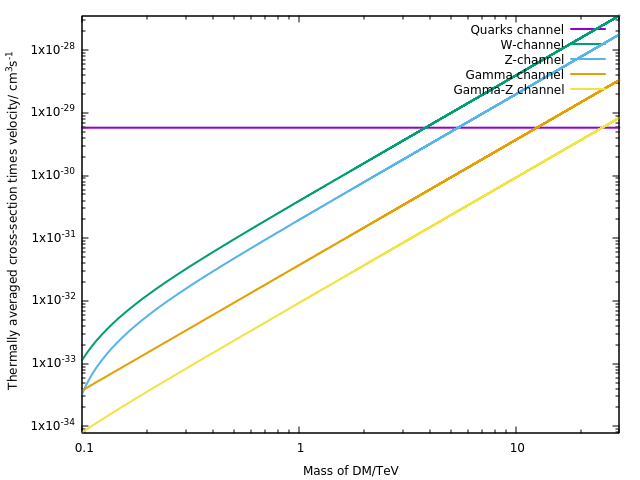
\includegraphics[scale=0.6]{CR1.png}\\
\textbf{Figue:} Thermally averaged cross-section times velocity versus the mass of the Dark Matter ranging from $100\; GeV$ to $30\; TeV$ 
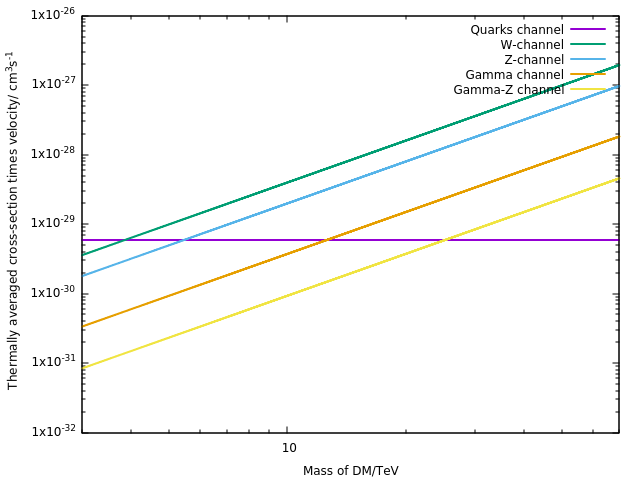
\includegraphics[scale=0.6]{CR2.png}\\
\textbf{Figue:} Thermally averaged cross-section times velocity versus the mass of the Dark Matter ranging from $3\; GeV$ to $70\; TeV$ 
\end{center}

From the figure, we estimate that below DM mass  $m_\chi \sim 3.7 TeV$ to $3.8 TeV$ quarks channel is relevant and above this range other particles. It should be noted here that this value depends on the couplings and the cut-off we set in our theory.\\
We get different patterns for different channels. We see that the quark channel remains almost constant. In this case, we recall that the mass dimension of our EFT operator was $5$.\\

But the other cross-section patterns show a rising behavior. It increases with the mass of our DM. It indicates the fact that EFT is non-renormalizable. If the mass becomes larger than the cut-off of our theory then it is not trusted. $\mathcal{O}_2$ and $\mathcal{O}_3$ were dimension $6$ operators.


\section{Discussion}
In this thesis paper, we commented on the annihilation cross-section times velocity for non-relativistic self-annihilating scalar dark matter in the framework of effective field theory and we demand that the mediators can not be produced on-shell.
In detail, we have discussed the motivation behind the dark matter. We have discussed the strong evidence of dark matter from observations. Then we mentioned the possible ways one can probe into the dark matter. We mentioned the characteristics of Dark Matter which we get from observations. This sets some constraints on EFT degrees of freedom. We considered WIMP as our DM candidate. Then we argued that WIMP i.e. weakly interacting massive particles, are potential DM candidates. We wanted to invoke our EFT in case of indirect detection. Therefore we derived the general formula for indirect detection. We noticed that this formula contains two parts, one we get from astrophysical observations and the other part, we get from the quantum field theory framework. We were interested in the latter. Then we constructed our EFT operators for the case of our singlet dark matter self-annihilating into standard model particles. We computed the thermally averaged cross-section times velocity which is almost equal to the cross-section times velocity as $T<<m_\chi$. We computed it for $q-channel, \; W-channel,\; Z-channel,\; \gamma-channel\; and\; \gamma Z-channel$. We found that all the cross-section contains $s-wave$ hence velocity is unsuppressed. Then we commented on the cross-section times velocity from this s-wave considering all couplings $0.5$, cutt-off $\Lambda= 100\; Tev$. As we suggested in our result that in different energy ranges signals of different channels are easier to detect.
From the graph of our results, we saw that how mass dimension $5$ and mass dimension $6$ operators behave. We saw that the quark channel was almost constant but the other channel was rising as the mass of the dark matter was rising. We already know about the non-renormalizability of EFT. Our result was evaluated by setting the cut-off $\Lambda=100\; TeV$ and we commented that above this mass range, our operators can not be trusted.

\chapter{Conclusion and Outlook}

In this thesis paper, we constructed standard model invariant effective operators in effective field theory framework for SM singlet i.e. real scalar Dark Matter self annihilating into standard model particles:$q\bar{q}$, $W^+ W^-$, $ZZ$, $\gamma\gamma$ and $\gamma\, Z$. We used this operator to compute annihilation cross-section times velocity which is almost equal to thermally averaged annihilation cross-section times velocity as $T<< m_\chi$. We discussed how these results can be used in the indirect detection of dark matter. We discussed how these results vary from each other setting all the couplings to $0.5$ and cutt-off $\Lambda=100 \; TeV$. We commented on the results of different channels and the effectiveness of our effective operators. The procedure we followed in this thesis is general. Following this method we can also compute photon flux for complex scalar dark matter, spin-1/2, and spin-1 dark matter. 


\begin{appendices}
\chapter{Feynman Rules}
To compute cross-sections for different cases we need to mention Feynman's rules for scalar fields, massive vector bosons, massless vector bosons, and fermions. We will not discuss it in detail but we will summarize all the rules we used here.

We need to specify here that W-boson and Z-boson are massive vectors, quarks are fermions, the photon is a massless vector field, DM candidate is a scalar field.

\textbf{Rules for scalar field:} First we need to draw all the connected parts of the initial and final states.
\begin{itemize}
\item In diagrams, scalar fields are drawn as dotted lines.
\item The external legs should be neglected i.e. they contribute $"1"$ to the amplitude.
\item To each vertex energy-momentum conservation should be imposed.
\item To each vertex, there is a corresponding vertex which we will compute.
\item To each internal line with momentum $p$ associate a propagator $$\tilde{G}(p) = \frac{i}{p^2-m^2+i \epsilon}$$
\item The four-momenta $k_i$ which are not fixed by energy-momentum conservation at each vertex should be integrated with a measure $\frac{d^4 k_i}{(2 \pi)^4}$.
\end{itemize} 

\textbf{Rules for fermions:}

\begin{itemize}
\item In diagrams, fermionic fields are drawn as solid lines.
\item To each vertex energy-momentum conservation should be imposed.
\item To each vertex, there is a corresponding vertex which we will compute.
\item Fermions with momentum towards the vertex are called incoming particles and momentum away from the vertex are called outgoing particles.
\item External line of incoming particle with momentum $p$ is represented by spinor $u(p)$.
\item External line of outgoing particle with momentum $p$ is represented by spinor $\bar{u}(p)$.
\item External line of incoming antiparticle with momentum $p$ is represented by $\bar{v}(p)$.
\item External line of outgoing antiparticle with momentum $p$ is represented by $v(p)$.

\item To each internal line with momentum $p$ associate a propagator $$\tilde{G}(p)= \frac{i}{\slashed{p}-m}$$
\end{itemize}


\textbf{Rules for massive vector fields:}

\begin{itemize}
\item In diagrams, massive vector fields are drawn as wiggly lines.
\item External line of incoming particle with momentum $p$ is represented by polarization vector $\epsilon^{(\lambda) \mu}$
\item External line of outgoing particle with momentum $p$ is represented by polarization vector $\epsilon^{(\lambda) \mu *}$
\item To each vertex energy-momentum conservation should be imposed.
\item To each vertex, there is a corresponding vertex which we will compute.
\item To each internal line with momentum $p$ associate %a propagator $$\tilde{G}(p) = \frac{-i(g^{\mu \nu}-\frac{p^\mu p^\nu}{m^2})}{p^2-m^2}$$.
\end{itemize}


\textbf{Rules for massless vector fields:}

\begin{itemize}
\item In diagrams, a massless vector field i.e. photon is drawn as wavy lines.
\item External line of incoming particle with momentum $p$ is represented by polarization vector $\epsilon^{(\lambda) \mu}$
\item External line of outgoing particle with momentum $p$ is represented by polarization vector $\epsilon^{(\lambda) \mu *}$
\item To each vertex energy-momentum conservation should be imposed.
\item To each vertex, there is a corresponding vertex which we will compute.
\item To each internal line with momentum $p$ associate a propagator $$\tilde{G}(p) = \frac{-ig^{\mu \nu}}{p^2}$$.
\end{itemize}

For a detailed derivation of these rules, one can consult \cite{pes}.

\end{appendices}







\begin{thebibliography}{}
\bibitem{rcurve}
 Y.~Sofue and V.~Rubin,
  ``Rotation curves of spiral galaxies,''
  Ann.\ Rev.\ Astron.\ Astrophys.\  {\bf 39}, 137 (2001)
  %doi:10.1146/annurev.astro.39.1.137
  [astro-ph/0010594].
  %%CITATION = doi:10.1146/annurev.astro.39.1.137;%%
  %491 citations counted in INSPIRE as of 08 Feb 2020

\bibitem {glensing}{}
J.~Rich [EROS-2 Collaboration],
  ``Limits on the Machos from EROS-2,''
  Nucl.\ Phys.\ Proc.\ Suppl.\  {\bf 173}, 40 (2007).
  %doi:10.1016/j.nuclphysbps.2007.08.021
  %%CITATION = doi:10.1016/j.nuclphysbps.2007.08.021;%%
  %1 citations counted in INSPIRE as of 08 Feb 2020


\bibitem {dmtheory1}{}
D.~Majumdar,
  ``Detection rates for Kaluza-Klein dark matter,''
  Phys.\ Rev.\ D {\bf 67}, 095010 (2003)
  %doi:10.1103/PhysRevD.67.095010
  [hep-ph/0209277].
  %%CITATION = doi:10.1103/PhysRevD.67.095010;%%
  %40 citations counted in INSPIRE as of 08 Feb 2020

\bibitem {dmtheory2}{}
Bertone, Gianfranco (edited),
``Particle Dark Matter: Observations, Models and                     Searches,''
Cambridge University Press, Cambridge, 2010

\bibitem {dmtheory3}{}
 W.~T.~Hu,
  ``Wandering in the Background: A CMB Explorer,''
  astro-ph/9508126.
  %%CITATION = ASTRO-PH/9508126;%%
  %100 citations counted in INSPIRE as of 08 Feb 2020

\bibitem {dmtheory4}{}
M.~Bauer and T.~Plehn,
  ``Yet Another Introduction to Dark Matter : The Particle Physics Approach,''
  Lect.\ Notes Phys.\  {\bf 959}, pp. (2019)
  %doi:10.1007/978-3-030-16234-4
  [arXiv:1705.01987 [hep-ph]].
  %%CITATION = doi:10.1007/978-3-030-16234-4;%%
  %31 citations counted in INSPIRE as of 08 Feb 2020

\bibitem {dmtheory6}{}
  S.~Profumo, L.~Giani and O.~F.~Piattella,
  ``An Introduction to Particle Dark Matter,''
  Universe {\bf 5}, no. 10, 213 (2019)
  %doi:10.3390/universe5100213
  [arXiv:1910.05610 [hep-ph]].
  %%CITATION = doi:10.3390/universe5100213;%%
  %1 citations counted in INSPIRE as of 08 Feb 2020
  
\bibitem{tasilecture}{}
  T.~R.~Slatyer,
  ``Indirect Detection of Dark Matter,''
  %doi:10.1142/9789813233348_0005
  arXiv:1710.05137 [hep-ph].
  %%CITATION = doi:10.1142/9789813233348_0005;%%
  %38 citations counted in INSPIRE as of 08 Feb 2020
  
\bibitem{kolbbook}{}
  E.~W.~Kolb and M.~S.~Turner,
  ``The Early Universe,''
  Front.\ Phys.\  {\bf 69}, 1 (1990).
  %%CITATION = FRPHA,69,1;%%
  %1772 citations counted in INSPIRE as of 08 Feb 2020

\bibitem{indtools}{}
 N.~L.~Rodd,
  ``Listening to the Universe through Indirect Detection,''
  arXiv:1805.07302 [hep-ph].
  %%CITATION = ARXIV:1805.07302;%%

\bibitem{eft1}{}
 A.~V.~Manohar,
  ``Introduction to Effective Field Theories,''
  arXiv:1804.05863 [hep-ph].
  %%CITATION = ARXIV:1804.05863;%%
  %29 citations counted in INSPIRE as of 08 Feb 2020
  
\bibitem{eft2}{}
 A.~Pich,
  ``Effective field theory: Course,''
  hep-ph/9806303.
  %%CITATION = HEP-PH/9806303;%%
  %285 citations counted in INSPIRE as of 08 Feb 2020

\bibitem{dmeft}{}
 S.~Liem, G.~Bertone, F.~Calore, R.~Ruiz de Austri, T.~M.~P.~Tait, R.~Trotta and C.~Weniger,
  ``Effective field theory of dark matter: a global analysis,''
  JHEP {\bf 1609}, 077 (2016)
  %doi:10.1007/JHEP09(2016)077
  [arXiv:1603.05994 [hep-ph]].
  %%CITATION = doi:10.1007/JHEP09(2016)077;%%
  %27 citations counted in INSPIRE as of 08 Feb 2020
  
\bibitem{whu}{}
http://background.uchicago.edu/~whu/intermediate/intermediate.html\\

\bibitem{plcol}{}
https://www.cosmos.esa.int/web/planck/publications\\


\bibitem{gwald}{}
Wald, Robert M.,
``General Relativity,''
Chicago Univ. Press, Chicago, USA, 1984
%doi:10.7208/chicago/9780226870373.001.0001


\bibitem{pcolab}{}
 N.~Aghanim {\it et al.} [Planck Collaboration],
  %``Planck 2018 results. VI. Cosmological parameters,''
  arXiv:1807.06209 [astro-ph.CO].
  %%CITATION = ARXIV:1807.06209;%%
  %2235 citations counted in INSPIRE as of 08 Feb 2020
  
\bibitem{pes}{}
Peskin, Michael E. and Schroeder, Daniel V.,
``An Introduction to quantum field theory,''
Addison-Wesley, Reading, USA, 1995


\end{thebibliography}

\end{document}
